\chapter{Desarrollo}

\section{Conocimientos previos y definiciones}
En esta sección se introducirán las nociones topológicas básicas para hacer autocontenido este trabajo. Dichas nociones nos darán el contexto y conocimientos necesarios para poder profundizar en el \emph{Teorema de Estabilidad} y ser capaces de abordar su demostración.

\subsection{Complejos Simpliciales}
Una forma de representar algunos espacios topológicos es a través de su descomposición en piezas más sencillas. Una descomposición de estas características se denomina complejo si sus piezas son topológicamente simples y sus intersecciones son piezas del mismo tipo, pero de dimensión inferior \cite{libroEH}. Existe una gran variedad de complejos con distintos grados de abstracción. En este trabajo nos centraremos en los complejos simpliciales, que permiten representar una gran variedad de espacios y son especialmente adecuados para cuestiones computacionales.

Los complejos simpliciales pueden ser estudiados desde un enfoque geométrico y desde un enfoque combinatorio. Partiremos de la definición de complejo simplicial desde el punto de vista geométrico. Para ello recordaremos algunos conceptos de geometría afín.

\begin{definition}
El conjunto de puntos $\{u_0, u_1, ..., u_k\}$ de $\mathbb{R}^d$ es \emph{afínmente independiente} si los vectores $\{\overrightarrow{u_0u_1}, ..., \overrightarrow{u_0u_k}\}$ son linealmente independientes.
\end{definition}

\begin{definition}
\begin{sloppypar}
Diremos que $x \in \mathbb{R}^d$ es \emph{combinación convexa} de los puntos ${u_0, u_1, ..., u_k}$ si $x = \sum_{i=0}^{k} \lambda_i u_i$ con $\lambda_i \geq 0 \ \text{ para todo } i \in \{0,...,k\}$ y $\sum_{i=0}^{k} \lambda_i = 1$.
\end{sloppypar}
\end{definition}

\begin{definition}
\begin{sloppypar}
Llamaremos \emph{envolvente convexa} de $u_0, u_1, ..., u_k$, denotado por ${\text{conv}\{u_0, u_1, ..., u_k\}}$, al conjunto de todas las combinaciones convexas de dichos puntos.
\end{sloppypar}
\end{definition}
Haciendo uso de este conjunto podremos definir nuestras piezas de la descomposición de la siguiente manera:

\begin{definition}
Un \emph{$k$\textit{-símplice}} $\sigma$ en $\mathbb{R}^d$ con $d \geq k$ es la envolvente convexa de $k+1$ puntos afínmente independientes  $u_0, u_1, ..., u_k \in \mathbb{R}^d$, es decir,
$\sigma \coloneqq \text{conv}\{u_0, u_1, ..., u_k\}$
\end{definition}

Diremos que el $k$-símplice $\sigma$ tiene dimensión $k$ y llamaremos \emph{vértices de $\sigma$} a los puntos $u_0, u_1, ..., u_k$.

\begin{figure}[h]
\centering
\begin{subfigure}[b]{0.2\textwidth}
\centering
   
\begin{tikzpicture}[thick, scale=0.7]
    	\tikzstyle{point}=[circle,thick,draw=black,fill=black,inner sep=0pt,minimum width=4pt,minimum height=4pt]
    	\node (a)[point] at (0,0) {};
    \end{tikzpicture}
    \caption{0-símplice}\label{ref:0simp}
\end{subfigure}
\begin{subfigure}[b]{0.2\textwidth}
\centering
	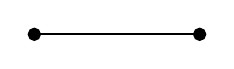
\begin{tikzpicture}[thick, scale=0.7]
    	\tikzstyle{point}=[circle,thick,draw=black,fill=black,inner sep=0pt,minimum width=4pt,minimum height=4pt]
    	\node (a)[point] at (0,0) {};
    	\node (b)[point] at (3,0) {};
 
    	\draw (a.center) -- (b.center) --cycle;
	\end{tikzpicture}
	\caption{1-símplice}\label{ref:1simp}
\end{subfigure}\hspace{0.05\textwidth}
\begin{subfigure}[b]{0.2\textwidth}
\centering
	\begin{tikzpicture}[thick, scale=3]
    	\tikzstyle{point}=[circle,thick,draw=black,fill=black,inner sep=0pt,minimum width=4pt,minimum height=4pt]
    	\coordinate (a) at (0,0);
    	\coordinate (b) at (1,0);
    	\coordinate (c) at (0.6,0.5);

    	\draw[fill=greeo,opacity=0.6] (a) -- (b) -- (c) -- cycle;
 
    	\draw (a) -- (b) -- (c)  --cycle;
    	
    	\node ()[point] at (a) {};
    	\node ()[point] at (b) {};
    	\node ()[point] at (c) {};
	\end{tikzpicture}
	\caption{2-símplice}\label{ref:2simp}
\end{subfigure}\hspace{0.05\textwidth}
\begin{subfigure}[b]{0.2\textwidth}
\centering
	\begin{tikzpicture}[thick,scale=3]
    	\tikzstyle{point}=[circle,thick,draw=black,fill=black,inner sep=0pt,minimum width=4pt,minimum height=4pt]

	\coordinate (A1) at (0,0);
	\coordinate (A3) at (1,0);
	\coordinate (A4) at (0.4,-0.3);
	\coordinate (B1) at (0.5,0.5);

	\draw[thick,dashed,opacity=0.6] (A1) -- (A3);
	\draw[fill=greeo,opacity=0.6] (A1) -- (A4) -- (B1) -- cycle;
	\draw[fill=greeo,opacity=0.6] (A3) -- (A4) -- (B1) -- cycle;

	\draw (A1) -- (B1)  -- (A3) -- (A4) --(A1) --cycle;
	
	\node ()[point] at (A1) {};
	\node ()[point] at (A3) {};
	\node ()[point] at (A4) {};
	\node ()[point] at (B1) {};
	\end{tikzpicture}
	\caption{3-símplice}\label{ref:3simp}
\end{subfigure}
\caption{Representación de los símplices de dimensión 0, 1, 2 y 3}
\end{figure}

Se puede observar que cualquier subconjunto de los vértices de $\sigma$ será afínmente independiente y por lo tanto definirá un símplice $\tau$ de dimensión inferior. De esta forma diremos que \emph{$\tau$ es una cara de $\sigma$} si es una combinación convexa de un subconjunto no vacío de los vértices de $\sigma$, y lo denotaremos por $\tau \leq \sigma$. Si el subconjunto es propio, diremos que \emph{$\tau$ es cara propia de $\sigma$}, y lo denotaremos por $\tau < \sigma$. Por otro lado, diremos que \emph{$\sigma$ es cocara (propia) de $\tau$}  si $\sigma \geq \tau$ ($\sigma > \tau$).

Haciendo uso de la definición de caras de un símplice $\sigma$ podemos definir \emph{el borde y el interior} de $\sigma$.

\begin{definition}
Sea $\sigma$ un símplice. Entonces
\begin{itemize}
	\item Se define el \emph{borde de $\sigma$} como \[\text{bd } \sigma = \bigcup_{\tau<\sigma}\tau\]
	\item Se define el \emph{interior de $\sigma$} como \[\text{int }\sigma= \sigma - \text{bd }\sigma\]
\end{itemize}
\end{definition}

\begin{remark}
Se sigue directamente de la definición que un punto $x \in \sigma$ pertenece al interior de $\sigma$ si y sólo si todos sus coeficientes $\lambda_i$ de la combinación convexa son positivos. Se sigue que cada punto $x \in \sigma$ pertenece únicamente al interior de la cara generada por los puntos con coeficientes $\lambda_i$ positivos.
\end{remark}

Una vez que ya conocemos las piezas de nuestra descomposición vamos a ver como tenemos que unirlas y cuáles son las principales propiedades de los complejos resultantes.\\
Como ya hemos visto al principio de la sección, para que una descomposición sea un complejo sus piezas tienen que ser topológicamente simples y sus intersecciones tienen que ser piezas de dimensión inferior del mismo tipo. La manera natural de hacer esto es pegar unos símplices con otros por sus caras.

\begin{definition}
Un \emph{complejo simplicial} es una colección finita de símplices $K$ que satisface las siguientes propiedades:
\begin{enumerate}
	\item Si $\sigma \in K$ y $\tau \leq \sigma$ entonces $\tau \in K$.
	\item Si $\sigma_0,\sigma_1 \in K$ y $\sigma_0 \cap \sigma_1 \neq \emptyset$ entonces $\sigma_0 \cap \sigma_1 \leq \sigma_i$ para $i = 1,2$.
\end{enumerate}
\end{definition}

Se define la dimensión de como el máximo de las dimensiones de sus símplices.

Un ejemplo de complejo simplicial es lo que se muestra en la figura \ref{ref:comp1}, mientras que en la figura \ref{ref:noComp} muestra un ejemplo que no es complejo simplicial.


\begin{figure}[ht]
\centering
\begin{tikzpicture}[thick,scale=3]
    	\tikzstyle{point}=[circle,thick,draw=black,fill=black,inner sep=0pt,minimum width=4pt,minimum height=4pt]

	\coordinate (x) at (0,0);

	\coordinate (A1) at (1,0);
	\coordinate (A3) at (2, 0.1);
	\coordinate (A4) at (1.4,-0.3);
	\coordinate (B1) at (1.5,0.5);

    \coordinate (b) at (3,0);
    \coordinate (c) at (2.6,-0.5);
    
    \coordinate (a1) at (3.4,0.12);
    \coordinate (b1) at (4,0);
    \coordinate (c1) at (3.8,0.3);
    
    \coordinate (y) at (3.5,-0.4);
	
	\draw[thick,dashed,opacity=0.6] (A1) -- (A3);
    \draw[fill=greeo,opacity=0.6] (a1) -- (b1) -- (c1) -- cycle;
	\draw[fill=greeo,opacity=0.6] (A1) -- (A4) -- (B1) -- cycle;
	\draw[fill=greeo,opacity=0.6] (A3) -- (A4) -- (B1) -- cycle;

	\draw (a1) -- (b1) -- (c1)  --cycle;	
	\draw (A1) -- (B1)  -- (A3) -- (A4) --(A1) --cycle;
	\draw (x) -- (A1) --cycle;	
	\draw (A3) -- (b) -- (c)  --cycle;	
	\draw (b1) -- (y) --cycle;
	\draw (B1) -- (A4) --cycle;
	
	\node ()[point] at (x) {};
	\node ()[point] at (A1) {};
	\node ()[point] at (A3) {};
	\node ()[point] at (A4) {};
	\node ()[point] at (B1) {};
    \node ()[point] at (b) {};
    \node ()[point] at (c) {};
    \node ()[point] at (a1) {};
    \node ()[point] at (b1) {};
    \node ()[point] at (c1) {};
    \node ()[point] at (y) {};	
	
	\end{tikzpicture}
\caption{Ejemplo de complejo simplicial}
\label{ref:comp1}
\end{figure}

\begin{figure}[ht]
\centering
\begin{tikzpicture}[thick]
    \tikzstyle{point}=[circle,thick,draw=black,fill=black,inner sep=0pt,minimum width=4pt,minimum height=4pt]
    \coordinate (a) at (0,0);
    \coordinate (b) at (3,0);
    \coordinate (c) at (2,2);

    \begin{scope}[yshift=2cm]
    	\coordinate (d) at (1,1);
    	\coordinate (e) at (0,2);
    	\coordinate (f) at (4,2);
    \end{scope}

	\coordinate (p) at (1.5,0.5);

    \draw[fill=greeo,opacity=0.6] (a) -- (b) -- (c) -- cycle;
    \draw[fill=greeo,opacity=0.6] (d) -- (e) -- (f) -- cycle;
    
 
    \draw (p) -- (d) --cycle;
    \draw (a) -- (b) -- (c)  --cycle;
    \draw (d) -- (e) -- (f) -- cycle;    
    
	\node ()[point] at (a) {};
    \node ()[point] at (b) {};
    \node ()[point] at (c) {};
    \node ()[point] at (d) {};
    \node ()[point] at (e) {};
    \node ()[point] at (f) {};
    \node ()[point] at (p) {};    
\end{tikzpicture}
\caption{Ejemplo de conjunto de símplices que no cumplen las condiciones de complejo simplicial}
\label{ref:noComp}
\end{figure}

\begin{definition}
El \emph{espacio subyacente} de un complejo simplicial $K$, denotado $\abs{K}$, es la unión de los símplices de $K$ con la topología heredada del $\mathbb{R}^d$ donde viven sus símplices. Este espacio subyacente también es llamado \emph{poliedro}.
\end{definition}
Como se puede observar, el espacio subyacente  de un complejo simplicial es compacto, siendo unión finita de símplices. El siguiente resultado caracteriza los abiertos y cerrados del espacio subyacente $\abs{K}$ de un complejo simplicial $K$.

\begin{proposition}
Sea $K$ un complejo simplicial y $A \subset \abs{K}$ un subconjunto. Entonces $A$ es un abierto (cerrado) en $K$ si y sólo si para cada $\sigma \in K$, $A \cap \abs{\sigma}$ es un abierto (cerrado) de $\abs{\sigma}$ \cite{libroEH}.
\end{proposition}

\begin{definition}
Una \emph{triangulación} de un espacio topológico $X$ es un par $(K, h)$ donde $K$ es un complejo simplicial y $h: X \to \abs{K}$ es un homeomorfismo ($h$ continua, biyectiva y $h^{-1}$ continua).
\end{definition}
Diremos que un espacio topológico es \emph{triangulable} si admite una triangulación.

También nos será de utilidad poder estudiar los complejos simpliciales contenidos en otro complejo simplicial.
\begin{definition}
Un \emph{subcomplejo} $L$ de un complejo simplicial $K$ es un complejo simplicial $L \subseteq K$.
\end{definition}

Un subcomplejo de gran interés son los \emph{$j$-esqueletos}, definidos de la siguiente forma: \[K^{(j)} = \{\sigma \in K \mid dim\ \sigma\ \leq j\}\]

Otro subconjunto de símplices que nos será de gran ayuda más adelante es la \emph{estrella de un símplice $\tau$}, la cual consiste de las cocaras de $\tau$, denotado por St $\tau$. Este conjunto no será siempre un complejo simplicial, así que se define la \emph{estrella cerrada} $\overline{\text{St}}\ \tau$ como el menor subcomplejo de $K$ que contiene a St $\tau$. Adicionalmente, se define el \emph{link} de $\tau$ como: $\text{Lk }\tau = \{v \in \overline{\text{St}}\ \tau \mid v \cap \tau = \emptyset\}$.

\subsubsection*{Complejos simpliciales abstractos}
Una vez que ya conocemos los complejos simpliciales desde el punto de vista geométrico, vamos a abordarlos desde un enfoque combinatorio, el cual nos será de gran ayuda para poder programar los complejos simpliciales.

\begin{definition}
Un \emph{complejo simplicial abstracto $A$} es una colección finita de conjuntos finitos tal que si $\alpha \in A$ y $\beta \subset \alpha$ entonces $\beta \in A$.
\end{definition}
De esta forma se cumple que
\begin{itemize}
	\item Los conjuntos en $A$ no vacíos se denominan \emph{símplices abstractos}.
	\item La \emph{dimensión} de un símplice abstracto $\alpha \in A$ es $\text{dim}\ \alpha = \text{card}(\alpha) - 1$. Y la dimensión del complejo es el máximo de las dimensiones de sus símplices.
	\item Una \emph{cara} de $\alpha \in A$ es cualquier subconjunto no vacío de $\beta \subset \alpha$.
	\item El \emph{conjunto de vértices} de $A$, denotado por $\text{Vert } A$, es la unión de todos sus símplices.
	\item Un \emph{subcomplejo $B$} de un complejo simplicial abstracto $A$ es un complejo simplicial abstracto $B \subset A$.
\end{itemize}

\begin{exmp}
Un ejemplo de complejo simplicial abstracto es el siguiente conjunto 

\begin{gather*}
A = \{\{0\},\{1\},\{2\},\{3\},\{4\},\{5\},\{6\},\{0,1\},\{1,2\},\{1,3\},\{1,4\},\{2,3\},\{2,4\},\{3,4\},\{4,5\},\\
\{4,6\},\{5,6\},\{1,2,3\},\{1,2,4\},\{1,3,4\},\{2,3,4\},\{1,2,3,4\}\}
\end{gather*}

Donde el conjunto de vértices es: $\text{Vert }A = \{0, 1, 2, 3, 4, 5, 6\}$.
\end{exmp}

\begin{definition}
Sean $A$ y $B$ dos complejos simpliciales abstractos. Diremos que $A$ y $B$ son \emph{isomorfos} si existe una biyección \[b:\text{Vert }A \to \text{Vert }B\] tal que $\alpha \in A$ si y sólo si $b(\alpha) \in B$.
\end{definition}

Cada complejo geométrico induce de manera natural un complejo abstracto de la siguiente forma:
\begin{definition}
Sea $K$ un complejo simplicial y $V$ el conjunto de vértices de $K$. Llamaremos \emph{esquema de vértices} al complejo simplicial abstracto $A$ formado por todos aquellos subconjuntos de $V$ que generan símplices en $K$.
\end{definition}

Y bajo ciertas circunstancias podremos hacer el paso opuesto de construir un complejo simplicial (geométrico) a partir de otro abstracto:
\begin{definition}
Sean $A$ un complejo simplicial abstracto y $K$ un complejo simplicial. Diremos que $K$ es una \emph{realización geométrica} de $A$, si $A$ es isomorfo al esquema de vértices de $K$.
\end{definition}

\begin{theorem}
Todo complejo simplicial abstracto de dimensión $d$ admite una realización geométrica en $\mathbb{R}^{2d + 1}$ \cite{libroEH}.
\end{theorem}

Así pues, los complejos simpliciales abstractos son una representación fiel de un complejo simplicial (geométrico).

\subsubsection*{Aplicaciones simpliciales}
Una vez que ya conocemos las principales propiedades de los complejos simpliciales, veremos cuales son las aplicaciones que preservan la estructura de complejo simplicial. Como vimos anteriormente, cada punto de un $k$-símplice pertenece al interior de exactamente una cara. Por lo tanto, todo punto $x \in \abs{K}$, siendo $K$ un complejo simplicial de vértices $u_0, u_1, ..., u_n$, pertenece al interior de uno de los símplices de $K$. Si $\sigma = \text{conv}\{u_0, u_1, ..., u_k\}$ es dicho símplice, entonces $x = \sum_{i=0}^{n} b_i(x)u_i$, donde
\[
b_i(x)=
\begin{cases}
\lambda_i	 & \text{ si } 0 \leq i \leq k \\ 
0 			 & \text{ si } k+1 \leq i \leq n
\end{cases},\text{ con } \lambda_i \text{ tal que } x = \sum_{i=0}^{k} \lambda_i u_i
\]
se denominan \emph{coordenadas baricéntricas} de $x$ en $K$.

Haremos uso de estas coordenadas para construir una función, lineal a trozos inducida por una función entre los vértices de dos complejos simpliciales, denominada \emph{aplicación de vértices}

\begin{definition}
Sean $K$ y $L$ complejos simpliciales y $\varphi:\text{Vert }K \to \text{Vert }L$ una aplicación. Diremos que $\varphi$ es una \emph{aplicación de vértices} si satisface que para cada $\sigma \in K$ su imagen $\varphi(\sigma) \in L$.
\end{definition}

Una aplicación de vértices $\varphi:\text{Vert }K \to \text{Vert }L$ induce una aplicación, lineal a trozos $f: \abs{K} \to \abs{L}$ dada por
\[
f(x) = f\left ( \sum_{i=0}^{n} b_i(x) u_i \right ) =  \sum_{i=0}^{n} b_i(x)u_i
\]
a la que llamaremos \emph{aplicación simplicial} asociada a $\varphi$. Para enfatizar que es una aplicación lineal en cada símplice del complejo, se suele notar la aplicación de la siguiente forma $f: K \to L$. 

\subsubsection*{Subdivisiones}
Veremos que hay ocasiones que nos interesará controlar el tamaño de los símplices de nuestro complejo simplicial conservando el espacio subyacente. Por esta razón, se introduce la noción de \emph{subdivisión de un complejo simplicial}.
\begin{definition}
Sea $K$ un complejo simplicial. Diremos que un complejo simplicial $L$ es una \emph{subdivisión} de $K$ si:
\begin{itemize}
	\item $\abs{K}=\abs{L}$.
	\item Cada símplice de $L$ está contenido en un símplice de $K$.
\end{itemize}
\end{definition}

Hay muchas maneras de obtener subdivisiones de un complejo simplicial, pero un tipo particular de subdivisión que es muy utilizada es la \emph{subdivisión baricéntrica}, denotada por $L = \text{Sd}K$. Para la construcción de esta subdivisión, introducimos el \emph{baricentro} de un símplice y el \emph{cono} de un símplice de vértice $v$.

\begin{definition}
Sea $\sigma$ un $k$-símplice, tal que $\sigma = \text{conv}\{v_0, v_1, ..., v_k\}$. Llamaremos \emph{baricentro} de $\sigma$ al punto
\[
b_\sigma = \sum_{i=0}^{k} \frac{v_i}{k+1}\ \in \text{int }\sigma
\]
\end{definition}

\begin{definition}
Sea $\sigma$ un $k$-símplice, tal que $\sigma = \text{conv}\{v_0, v_1, ..., v_k\}$ y $v$ un punto no contenido en el subespacio afín generado por $\{v_0, v_1, ..., v_k\}$. Se define el \emph{cono} de $\sigma$ con vértice $v$ y se denota por $\sigma*v$ como el $k+1$-símplice generado por $\{v,v_0, v_1, ..., v_k\}$.
\end{definition}

\begin{definition}
Sea $K$ un complejo simplicial. Se define la \emph{subdivisión baricéntrica} de $K$ como el complejo simplicial Sd$K$ que se construye inductivamente sobre el $j$-esqueleto como sigue:
\begin{enumerate}
	\item Sd$K^{(0)} = K^{(0)}$.
	\item Sd$K^{(j)}$ es la unión de Sd$K^{(j-1)}$ con el conjunto de todos los símplices de la forma $b_\sigma*\tau$, donde $\sigma$ es un $j$-símplice y $\tau$ es cualquier símplice de Sd$K^{(j-1)}$ contenido en una cara de $\sigma$.
\end{enumerate}
\end{definition}
En la figura \ref{ref:subBar} se muestra la primera y segunda subdivisión baricéntrica de un complejo simplicial.

\begin{figure}[h]
\centering
\begin{subfigure}[b]{0.3\textwidth}
\centering
	\begin{tikzpicture}[thick, scale=4]
    	\tikzstyle{point0}=[circle,thick,draw=black,fill=black,inner sep=0pt,minimum width=4pt,minimum height=4pt]
    	
    	\coordinate (a) at (0,0);
    	\coordinate (b) at (1,0);
    	\coordinate (c) at (0.5,0.7);

    	\draw[fill=greeo,opacity=0.6] (a) -- (b) -- (c) -- cycle;
 
    	\draw (a) -- (b) -- (c)  --cycle;
    	
    	\node ()[point0] at (a) {};
    	\node ()[point0] at (b) {};
    	\node ()[point0] at (c) {};
	\end{tikzpicture}
	\caption{2-símplice}\label{ref:2simpBar}
\end{subfigure}\hspace{0.02\textwidth}
\begin{subfigure}[b]{0.3\textwidth}
\centering
	\begin{tikzpicture}[thick, scale=4]
    	\tikzstyle{point0}=[circle,thick,draw=black,fill=black,inner sep=0pt,minimum width=4pt,minimum height=4pt]
    	\tikzstyle{point1}=[circle,thick,draw=black,fill=red,inner sep=0pt,minimum width=4pt,minimum height=4pt]
    	
    	\coordinate (a) at (0,0);
    	\coordinate (b) at (1,0);
    	\coordinate (c) at (0.5,0.7);
    	\coordinate (d) at (0.25,0.35);
    	\coordinate (e) at (0.5,0);
    	\coordinate (f) at (0.75,0.35);
    	\coordinate (g) at (0.5,0.23);

		\draw[fill=greeo,opacity=0.6] (a) -- (b) -- (c) -- cycle;
		
    	\draw (a) -- (b) -- (c)  --cycle;
    	\draw (a) -- (f) --cycle;
    	\draw (c) -- (e) --cycle;
    	\draw (d) -- (b) --cycle;
    	
		\node ()[point0] at (a) {};
		\node ()[point0] at (b) {};
		\node ()[point0] at (c) {};   
    	\node ()[point1] at (d) {};
    	\node ()[point1] at (e) {};
    	\node ()[point1] at (f) {};
    	\node ()[point1] at (e) {};
    	\node ()[point1] at (g) {};
	\end{tikzpicture}
	\caption{Primera subdivisión baricéntrica}\label{ref:1SubBar}
\end{subfigure}\hspace{0.02\textwidth}
\begin{subfigure}[b]{0.3\textwidth}
\centering
	\begin{tikzpicture}[thick, scale=4]
    	\tikzstyle{point0}=[circle,thick,draw=black,fill=black,inner sep=0pt,minimum width=4pt,minimum height=4pt]
    	\tikzstyle{point1}=[circle,thick,draw=black,fill=red,inner sep=0pt,minimum width=4pt,minimum height=4pt]
    	\tikzstyle{point2}=[circle,thick,draw=black,fill=blue,inner sep=0pt,minimum width=4pt,minimum height=4pt]
    	
    	\coordinate (a) at (0,0);
    	\coordinate (b) at (1,0);
    	\coordinate (c) at (0.5,0.7);
    	\coordinate (d) at (0.25,0.35);
    	\coordinate (e) at (0.5,0);
    	\coordinate (f) at (0.75,0.35);
    	\coordinate (g) at (0.5,0.23);
    	\coordinate (h) at (0.38,0.53);
    	\coordinate (i) at (0.5,0.47);
    	\coordinate (j) at (0.63,0.53);
    	\coordinate (k) at (0.38,0.29);
    	\coordinate (l) at (0.63,0.29);
    	\coordinate (m) at (0.42,0.43);
    	\coordinate (n) at (0.58,0.43);
    	\coordinate (o) at (0.13,0.18);
    	\coordinate (p) at (0.25,0.12);
    	\coordinate (q) at (0.5,0.12);
    	\coordinate (r) at (0.25,0);
    	\coordinate (s) at (0.25,0.19);
    	\coordinate (t) at (0.33,0.08);
    	\coordinate (u) at (0.88,0.18);
    	\coordinate (v) at (0.75,0.12);
    	\coordinate (w) at (0.75,0);
    	\coordinate (x) at (0.67,0.08);
    	\coordinate (y) at (0.75,0.19);

		\draw[fill=greeo,opacity=0.6] (a) -- (b) -- (c) -- cycle;
		
    	\draw (a) -- (b) -- (c)  --cycle;
    	\draw (a) -- (f) --cycle;
    	\draw (c) -- (e) --cycle;
    	\draw (d) -- (b) --cycle;
    	\draw (c) -- (k) --cycle;
    	\draw (g) -- (h) --cycle;
    	\draw (d) -- (i) --cycle;
    	\draw (c) -- (l) --cycle;
    	\draw (g) -- (j) --cycle;
    	\draw (f) -- (i) --cycle;
    	\draw (a) -- (k) --cycle;
    	\draw (d) -- (p) --cycle;
    	\draw (g) -- (o) --cycle;
    	\draw (g) -- (r) --cycle;
    	\draw (e) -- (p) --cycle;
    	\draw (a) -- (q) --cycle;
    	\draw (e) -- (v) --cycle;
    	\draw (b) -- (q) --cycle;
    	\draw (g) -- (w) --cycle;
    	\draw (b) -- (l) --cycle;
    	\draw (g) -- (u) --cycle;
    	\draw (f) -- (v) --cycle;
    	
		\node ()[point0] at (a) {};
		\node ()[point0] at (b) {};
		\node ()[point0] at (c) {};   
    	\node ()[point1] at (d) {};
    	\node ()[point1] at (e) {};
    	\node ()[point1] at (f) {};
    	\node ()[point1] at (e) {};
    	\node ()[point1] at (g) {};
    	\node ()[point1] at (f) {};
    	\node ()[point1] at (g) {};
    	\node ()[point2] at (h) {};
    	\node ()[point2] at (i) {};
    	\node ()[point2] at (j) {};
    	\node ()[point2] at (k) {};
    	\node ()[point2] at (l) {};
    	\node ()[point2] at (m) {};
    	\node ()[point2] at (n) {};
    	\node ()[point2] at (o) {};
    	\node ()[point2] at (p) {};
    	\node ()[point2] at (q) {};
    	\node ()[point2] at (r) {};
    	\node ()[point2] at (s) {};
    	\node ()[point2] at (t) {};
    	\node ()[point2] at (u) {};
    	\node ()[point2] at (v) {};
    	\node ()[point2] at (w) {};
    	\node ()[point2] at (x) {};
    	\node ()[point2] at (y) {};
	\end{tikzpicture}
	\caption{Segunda subdivisión baricéntrica}\label{ref:2SubBar}
\end{subfigure}
\caption{Primera y segunda subdivisión baricéntrica de un 2-símplice}
\label{ref:subBar}
\end{figure}

Recordemos que el \emph{diámetro} de un subconjunto $A \subset \mathbb{R}^d$ es el supremo sobre las distancias entre sus puntos. 

\begin{lemma}
Si $\sigma$ es un $k$-símplice, entonces el diámetro de cada símplice en la subdivisión baricéntrica de $\sigma$ es como máximo $\frac{k}{k+1}\text{diam }\sigma$ \cite{libroEH}. 
\end{lemma}

De forma que gracias al lema anterior podremos hacer el diámetro de los símplices de los complejos simpliciales tan pequeño como queramos, ya que el diámetro de los símplices de la $n$-ésima subdivisión baricéntrica del complejo simplicial $K$, denotado por $\text{Sd}^nK = \text{Sd}(\text{Sd}^{n - 1}K)$, es 
\[
\left ( \frac{k}{k+1} \right )^n \text{diam } \sigma  \underset{n \to \infty}{\longrightarrow} 0,\ con\ \sigma \in K \text{ y } k = \text{dim } \sigma
\]

\subsubsection*{Aproximaciones simpliciales}
Para estudiar la topología de los poliedros es fundamental aproximar funciones continuas por aplicaciones simpliciales. Para poder definir estas aproximaciones primero vamos a definir un tipo de entorno de los vértices de un complejo como se puede ver en la figura \ref{ref:entEstrellado}.

\begin{definition}
Sea $K$ un complejo simplicial y $v$ un vértice de $K$. El conjunto
\[
N(v) = \bigcup_{\sigma \in \text{St } v} \text{int }\sigma
\]
es un entorno abierto de $v$ en $\abs{K}$ al que llamaremos \emph{entorno estrellado} de $v$.
\end{definition}

\begin{figure}[h]
\centering
	\begin{tikzpicture}[thick, scale=4]
    	\tikzstyle{point}=[circle,thick,draw=black,fill=black,inner sep=0pt,minimum width=4pt,minimum height=4pt]

    	
    	\coordinate (a) at (0,0);
    	\coordinate (b) at (1,0);
    	\coordinate (c) at (0.5,0);
    	\coordinate (d) at (0.5,0.5);
    	\coordinate (e) at (0.5,-0.5);
    	\coordinate (f) at (1.29,0.44);
    	\coordinate (g) at (1.5,-0.49);
    	\coordinate (h) at (1.02,-0.64);
    	
		\node ()[point] at (c) {};		
		
		\draw[fill=greeo,opacity=0.6] (e) -- (h) -- (g) -- (f) -- (d) -- (b) -- cycle;
				
    	\draw (a) -- (d) -- (f)  -- (g) -- (h) -- (e) --cycle;
    	\draw (a) -- (b) --cycle;
    	\draw (d) -- (e) --cycle;
    	\draw (b) -- (f) --cycle;
    	\draw (b) -- (g) --cycle;
    	\draw (b) -- (h) --cycle;
    
    	\draw[fill=redp,opacity=0.6] (a) -- (d) -- (b) -- (e) -- cycle;
    	
		\node ()[point] at (a) {};
		\node ()[point] at (b) {};
		\node ()[label={[shift={(0.2,-0.15)}]\small $v$}] at (c) {};
    	\node ()[point] at (d) {};
    	\node ()[point] at (e) {};
    	\node ()[point] at (f) {};
    	\node ()[point] at (e) {};
    	\node ()[point] at (g) {};
    	\node ()[point] at (h) {};
    	\node () at (0.35,0.17) {$N(v)$};
	\end{tikzpicture}
\caption{Entorno estrellado de $v$ marcado en color rojo}
\label{ref:entEstrellado}
\end{figure}

Así pues, definimos una aproximación simplicial de la siguiente forma:
\begin{definition}
Sean $K$ y $L$ complejos simpliciales, $g: \abs{K} \to \abs{L}$ una aplicación continua y  $f: K \to L$ una aplicación simplicial. Diremos que $f$ es una \emph{aproximación simplicial} de $g$ si verifica la \emph{condición de estrella}, es decir, si para cada vértice $v \in K$ se tiene que $g(N(v)) \subset N(f(v))$.
\end{definition}

Además, la condición de estrella será una condición suficiente para garantizar la existencia de una aproximación simplicial:
\begin{lemma}
Sean $K$ y $L$ complejos simpliciales, $g: \abs{K} \to \abs{L}$ una aplicación continua que satisface la condición de estrella. Entonces $g$ tiene una aproximación simplicial $f: K \to L$ \cite{libroEH}.
\end{lemma}

En la figura \ref{ref:aproxSimp} podemos ver un ejemplo de aproximación simplicial de una aplicación continua.

\begin{figure}[!ht]
\centering
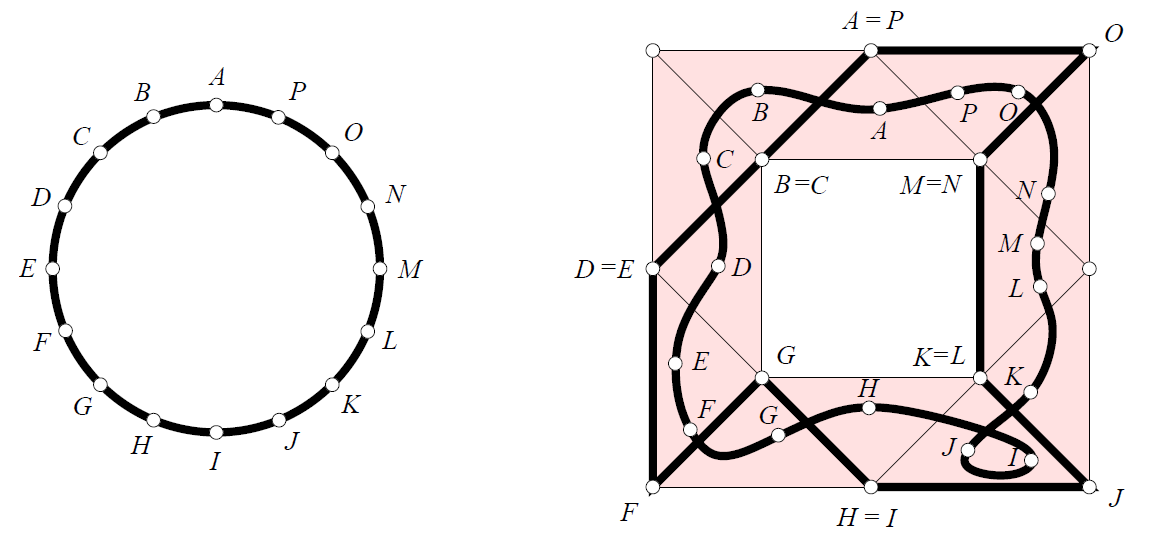
\includegraphics[width=0.8\textwidth]{include/figuras/aproximacionSimplicial.png} 
\caption{Aplicación continua del círculo en una corona circular y una aproximación simplicial de dicha aplicación. Fuente: \cite{libroEH}}
\label{ref:aproxSimp}
\end{figure}

\begin{theorem}[Aproximación simplicial]
\label{ref:teoremaAproximacionSimplicial}
\begin{sloppypar}
Sean $K$ y $L$ complejos simpliciales, ${g: \abs{K} \to \abs{L}}$ una aplicación continua. Entonces existe $n \in \mathbb{N}$ tal que $g$ tiene una aproximación simplicial ${f: \textit{Sd}^{n}\ K \to L}$  \cite{libroEH}.
\end{sloppypar}
\end{theorem}

\subsection{Complejos simpliciales de nubes de puntos}
Desde el punto de vista computacional nos encontramos con el problema de que tenemos una representación de un espacio topológico a través de una discretización finita de los puntos de dicho espacio, y nuestro objetivo es poder recuperar propiedades del espacio topológico original a partir de esta nube de puntos. Para ello asociaremos complejos simpliciales a dicha nube de puntos.

\subsubsection*{Complejo de \v{C}ech}
El complejo de \v{C}ech se define a partir de la intersección de una colección de circunferencias. Por lo que primero estudiaremos como podemos obtener un complejo simplicial a partir de la intersección de una colección finita de conjuntos.

\begin{definition}
Sea $F$ una colección finita de conjuntos. Se define el \emph{nervio} de F como el complejo simplicial abstracto
\[
\text{Nrv }F= \left\{ X \subseteq F \mid \bigcap X \neq \emptyset \right\}
\]
\end{definition}

Consideramos el caso particular en el que los conjuntos de la familia son las bolas cerradas $\overline{B}_r(x)= \{y\in \mathbb{R}^d \mid d(x,y) \leq r\}$ en $\mathbb{R}^d$.

\begin{figure}[!ht]
\centering
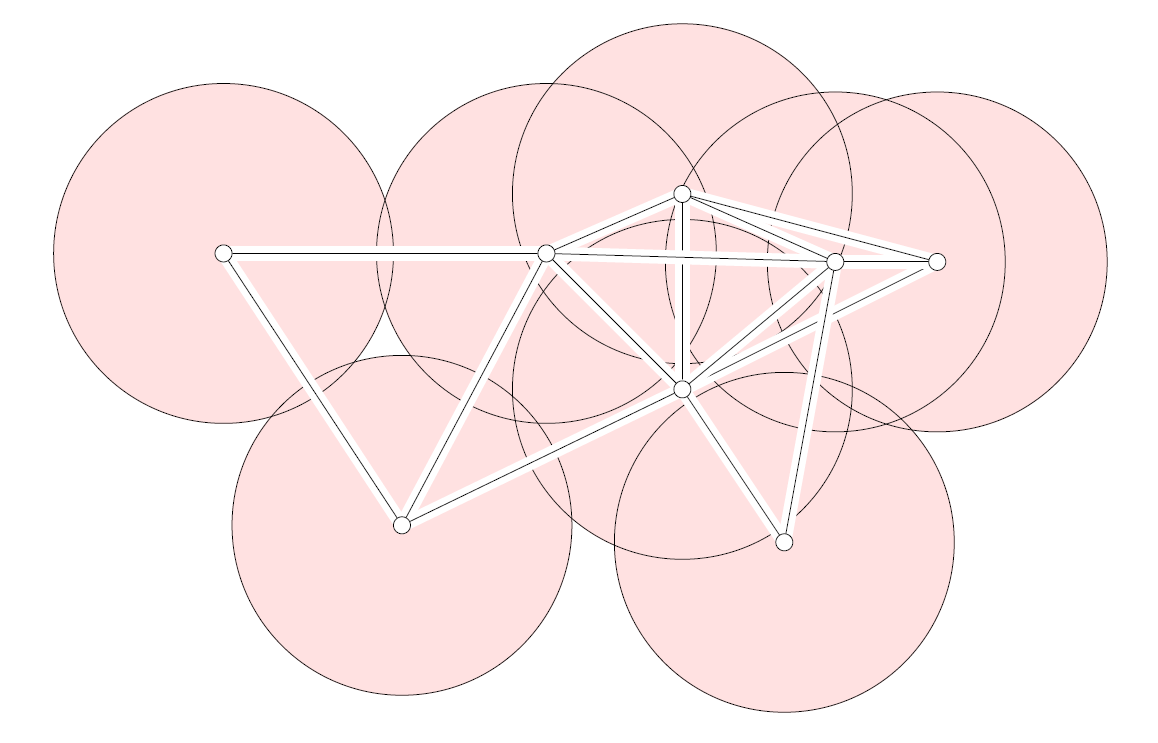
\includegraphics[width=0.5\textwidth]{include/figuras/Cech.png} 
\caption{Complejo de \v{C}ech para un conjunto de nueve puntos y un radio $r$. Fuente: \cite{libroEH}}
\label{ref:cech}
\end{figure}

\begin{definition}
Sea $S\subset \mathbb{R}^d$ un conjunto finito de puntos. Llamaremos \emph{complejo de \v{C}ech} de $S$ de radio $r$ al complejo simplicial abstracto
\[
\text{\v{C}ech}(r)=\left\{\sigma \subset S \mid \bigcap_{u \in \sigma} \overline{B}_r(u)\neq \emptyset \right\}
\]
\end{definition}

El complejo de \v{C}ech es isomorfo al nervio del conjunto de las bolas cerradas de radio $r$ centrada en los puntos de $S$. En la figura \ref{ref:cech} podemos observar un ejemplo de complejo de \v{C}ech.

Podemos comprobar \cite{libroEH} que para valores de $r$ lo suficientemente grandes, $\text{\v{C}ech}(r)$ es un símplice de dimensión $\text{card}(S)-1$. Lo cual, va a hacer que el complejo de \v{C}ech sea poco eficiente desde el punto de vista computacional.\\
Además, en general, el complejo de \v{C}ech de un conjunto de puntos $S \subset \mathbb{R}^d$ no posee una realización geométrica en $\mathbb{R}^d$.



\subsubsection*{Complejo de Vietoris-Rips}

\begin{definition}
Sea $S \subset \mathbb{R}^d$ un conjunto finito de puntos. Llamamos \emph{complejo de Vietoris-Rips} de $S$ de radio $r$ al complejo simplicial abstracto
\[
\text{VR}(r) = \{\sigma \subseteq  S \mid \text{diam } \sigma \leq 2r\}
\]
\end{definition}

En la figura \ref{ref:vr} podemos observar como se generan los diversos complejos de VR a medida que se va aumentando el radio.

\begin{figure}[!ht]
\centering
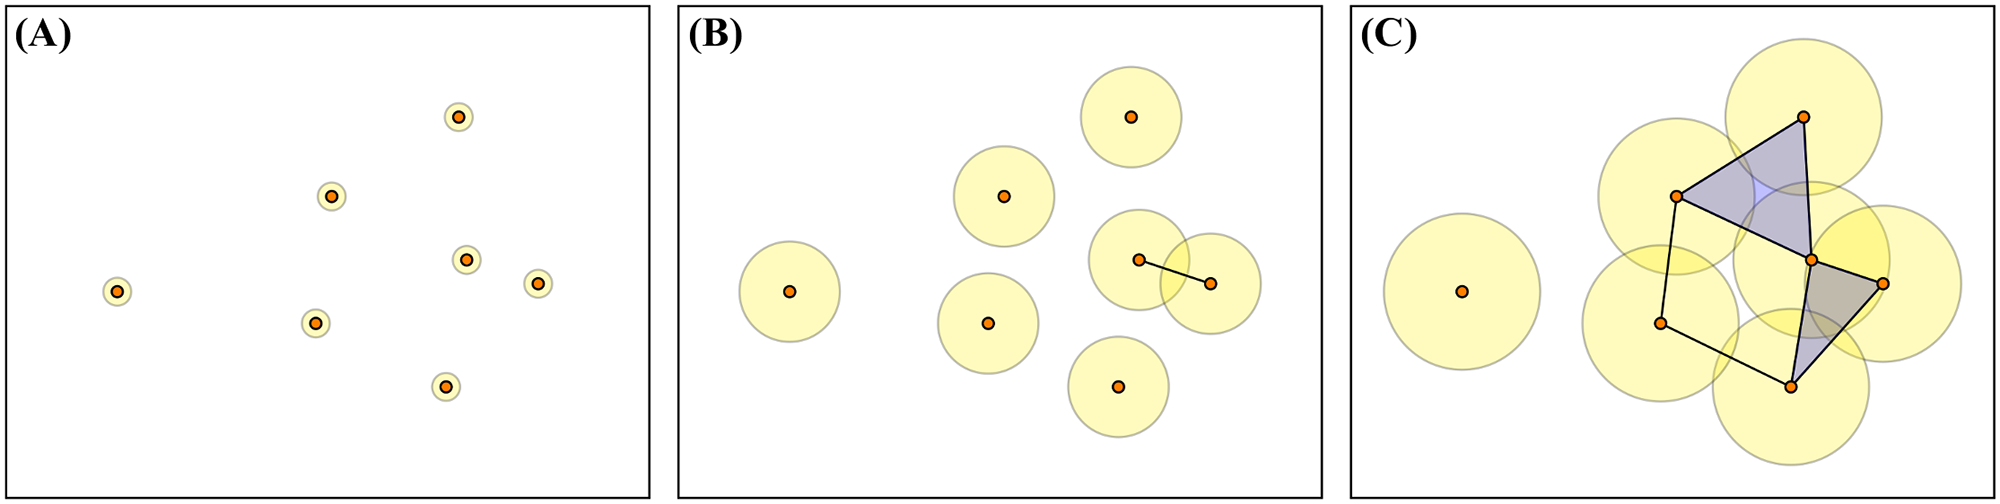
\includegraphics[width=0.9\textwidth]{include/figuras/vr.png} 
\caption{Complejos de Vietoris-Rips para un conjunto de siete puntos a medida que aumentamos el radio de izquierda a derecha. Fuente: \cite{Ulmer2019}}
\label{ref:vr}
\end{figure}

Sea $\sigma \subset S$, entonces $\text{diam } \sigma = \max\limits_{u, v \in \sigma} d(u,v)$. Esta observación garantiza que $\sigma \in \text{VR}(r)$ si y sólo si todas sus aristas están en $\text{VR}(r)$. Dicho de otro modo, $\text{VR}(r)$ está completamente determinado por su $1$-esqueleto. Esto hace que el complejo de Vietoris-Rips sea mucho más eficiente que el complejo de \v{C}ech desde el punto de vista computacional. Sin embargo, al igual que ocurre con el complejo de \v{C}ech, no admite una realización geométrica en $\mathbb{R}^d$.

Por otro lado, el complejo de Vietoris-Rips no es el nervio de ningún recubrimiento. Sin embargo, el siguiente resultado garantiza que el complejo de VR aproxima al complejo de \v{C}ech.

\begin{lemma}[Lema de Vietoris-Rips]
\label{ref:lemaVR}
Sea $S \subset \mathbb{R}^d$ un conjunto finito de puntos y sea $r \geq 0$. Entonces,
\[
\text{\v{C}ech}(r) \subset \text{VR}(r) \subset \text{\v{C}ech}(\sqrt{2}r)
\]
\end{lemma}

La demostración al lema \ref{ref:lemaVR} se puede encontrar en \cite{libroEH}.

\subsubsection*{Complejo de Delaunay}
En esta sección introduciremos construcciones geométricas que nos limitarán la dimensión de los símplices que obtenemos del nervio de una colección finita de conjuntos.

\begin{definition}
Sea $S \subset \mathbb{R}^d$ un conjunto finito. Se define la \emph{celda de Voronoi} de un punto $u \in S$ como el conjunto de los puntos
\[
V_u = \{ x \in \mathbb{R}^d \mid d(x,u) \leq d(x,v) \forall v \in S\}
\]
La colección de las celdas de Voronoi de los puntos de $S$ se denomina \emph{diagrama de Voronoi} de $S$.
\end{definition}

En la figura \ref{ref:vor-del} se puede ver el diagrama de Voronoi de un conjuntos de puntos. Nótese que las celdas de Voronoi recubren todo el espacio.

\begin{definition}
Sea $S \subset \mathbb{R}^d$ un conjunto finito. Se define el \emph{complejo de Delaunay} de $S$ como el complejo simplicial abstracto 
\[
\text{Del} = \left\{\sigma \subseteq S \mid \bigcap_{u \in \sigma}V_u \neq \emptyset \right\}
\] 
\end{definition}

El complejo de Delaunay es un complejo isomorfo al nervio del diagrama de Voronoi. Además, si los puntos de $S$ están en posición general, se obtiene una realización del complejo de Delauney en $\mathbb{R}^d$ considerando envolventes convexas de los símplices abstractos. Esta realización geométrica se denomina \emph{triangulación de Delaunay}.

\begin{figure}[!ht]
\centering
\begin{subfigure}[b]{0.4\textwidth}
	\centering
	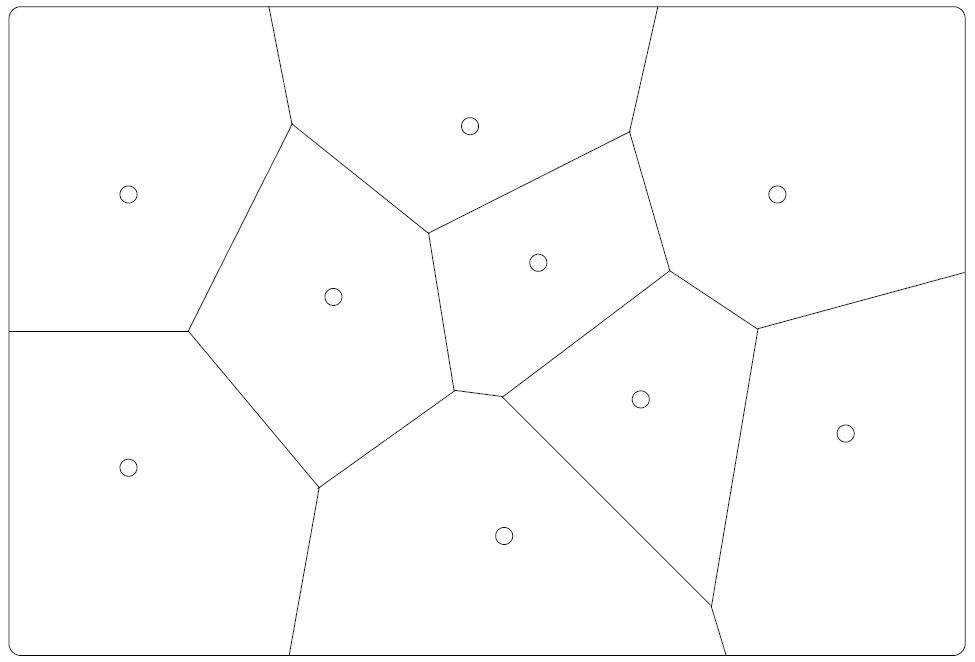
\includegraphics[width=0.9\textwidth]{include/figuras/voronoi.png} 
\end{subfigure}
\begin{subfigure}[b]{0.4\textwidth}
	\centering
	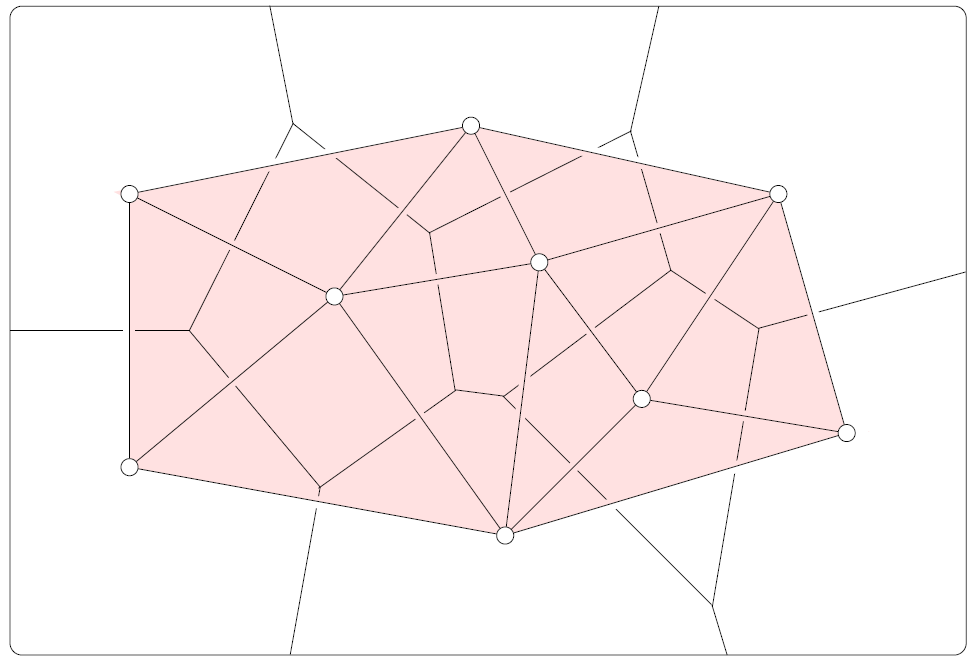
\includegraphics[width=0.9\textwidth]{include/figuras/delaunay.png} 
\end{subfigure}
\caption{A la izquierda tenemos el Diagrama de Voronoi de un conjunto de nueve puntos en el plano, y a la derecha triangulación de Delaunay superpuesta al diagrama de Voronoi. Fuente: \cite{libroEH}}
\label{ref:vor-del}
\end{figure}

\subsubsection*{Alfa complejo}
Sea $S \subset \mathbb{R}^d$ un conjunto finito de puntos y $r \geq 0$. Para cada $u \in S$ consideramos la región $R_u(r)= \overline{B}_r(u) \cap V_u$, es decir, la intersección de la región de Voronoi de $u$ con la bola cerrada de centro $u$ y radio $r$.

\begin{definition}
Sea $S \subset \mathbb{R}^d$ un conjunto finito de puntos y $r \geq 0$.Se define el \emph{Alfa complejo} de radio $r$ asociado a $S$ como el complejo simplicial abstracto
\[
\text{Alpha}(r)=\left\{\sigma \in S \mid \bigcap_{u \in \sigma}R_u(r) \neq \emptyset \right\}
\]
\end{definition}

En la figura \ref{ref:alpha} se puede observar la unión de dichas regiones y su correspondiente alfa complejo. Se puede observar que el alfa complejo es isomorfo al nervio de la colección formada por los $R_u(r)$.

\begin{figure}[!ht]
\centering
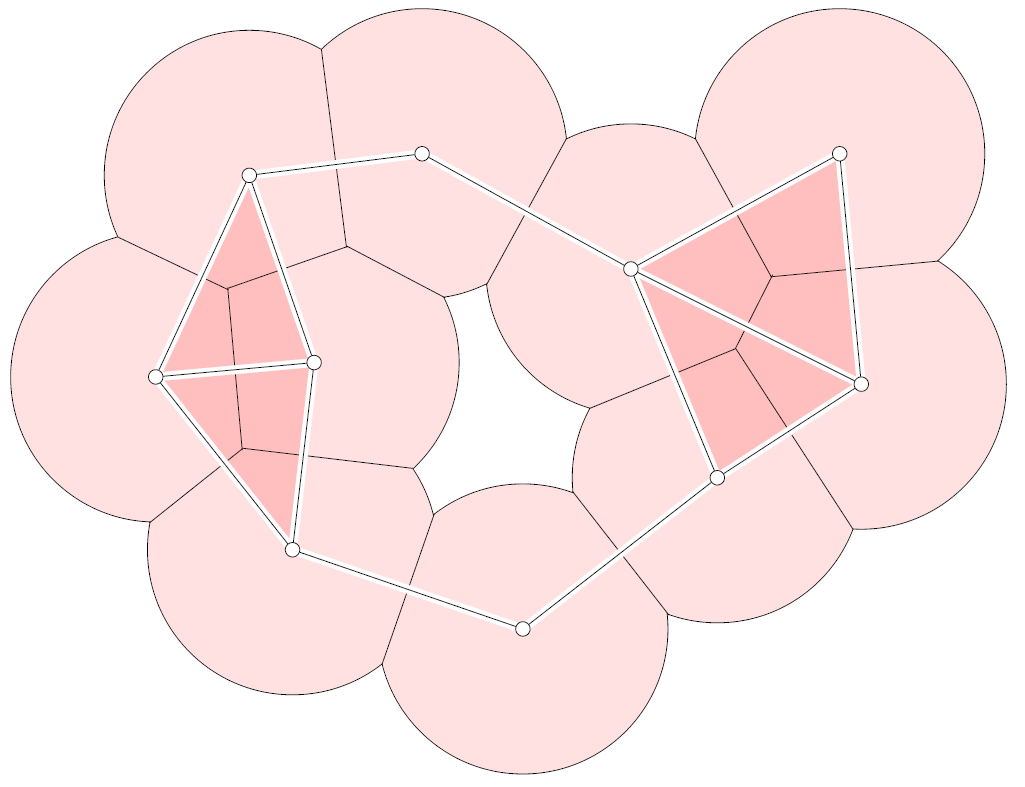
\includegraphics[width=0.5\textwidth]{include/figuras/alpha.png} 
\caption{Unión de las regiones $R_u(r)$ asociadas a un radio $r$ y un conjunto finito de puntos $S$. El correspondiente alfa complejo es superpuesto a esta unión de regiones. Fuente: \cite{libroEH}}
\label{ref:alpha}
\end{figure}

Puesto que $R_u(r) \subset \overline{B}_r(u)$ para cada $u \in S$, se tiene que $\text{Alpha}(r) \subset \text{\v{C}ech}(r)$. Del mismo modo, dado que $R_u(r) \subset V_u$ para cada $u \in S$, se tiene que $\text{Alpha}(r) \subset \text{Del}(S)$.

Además el alfa complejo tiene menos símplices que el complejo de \v{C}ech. Y como es un subcomplejo del complejo de Delaunay, admite de manera natural una realización en $\mathbb{R}^d$. Por lo que hace que los alfa complejos sean una buena opción desde el punto de vista computacional.


\subsection{Homología}
Como se puede ver en [añadir cita] la homotopía es una potente herramienta algebraica para poder obtener propiedades de los espacios topológicos. Sin embargo, los métodos para el cálculo de la homotopía no son manejables computacionalmente. Así pues, se propone la homología como formalismo algebraico, que, aunque no es capaz de obtener tanta información topológica sobre el espacio como con otros formalismos, es muy computable.

Comenzaremos estudiando los diversos grupos que están involucrados en la definición de la homología.

\subsubsection*{Grupos de cadenas}
Sea $K$ un complejo simplicial y $p$ un número entero no negativo. Una \emph{$p$-cadena} en $K$ es una suma formal de $p$-símplices en $K$. Más concretamente, $c$ es una $p$-cadena en $K$ si
\[
c = \sum a_i\sigma_i
\]
con $\sigma_i$ es un $p$-símplice para cada $i$ y $a_i$ son los \emph{coeficientes}. Estos coeficientes pueden tomarse de cualquier anillo conmutativo, sin embargo, nosotros usaremos con coeficientes en el cuerpo de dos elementos, es decir, $a_i \in \mathbb{Z}_2$. 

\begin{exmp}
Escribiremos los símplices como la lista de sus vértices, $\sigma = [u_0, u_1, ..., u_p]$.
\begin{itemize}
	\item En la figura \ref{ref:0cad} se muestra en rojo la $0$-cadena $c=[0]+[2]+[6]+[9]$.
\begin{figure}[!ht]
\centering
\begin{tikzpicture}[thick,scale=3]
    	\tikzstyle{point}=[circle,thick,draw=black,fill=black,inner sep=0pt,minimum width=4pt,minimum height=4pt]
    	\tikzstyle{point1}=[circle,thick,draw=black,fill=red,inner sep=0pt,minimum width=7pt,minimum height=7pt]

	\coordinate (x) at (0,0);

	\coordinate (A1) at (1,0);
	\coordinate (A3) at (2, 0.1);
	\coordinate (A4) at (1.4,-0.3);
	\coordinate (B1) at (1.5,0.5);

    \coordinate (b) at (3,0);
    \coordinate (c) at (2.6,-0.5);
    
    \coordinate (a1) at (3.4,0.12);
    \coordinate (b1) at (4,0);
    \coordinate (c1) at (3.6,0.3);
    
    \coordinate (y) at (3.5,-0.4);
	
	\draw[thick,dashed,opacity=0.6] (A1) -- (A3);
    \draw[fill=greeo,opacity=0.6] (b) -- (b1) -- (c1) -- cycle;
	\draw[fill=greeo,opacity=0.6] (A1) -- (A4) -- (B1) -- cycle;
	\draw[fill=greeo,opacity=0.6] (A3) -- (A4) -- (B1) -- cycle;

	\draw (b) -- (b1) -- (c1)  --cycle;	
	\draw (A1) -- (B1)  -- (A3) -- (A4) --(A1) --cycle;
	\draw (x) -- (A1) --cycle;	
	\draw (A3) -- (b) -- (c)  --cycle;	
	\draw (b1) -- (y) --cycle;
	\draw (B1) -- (A4) --cycle;	
	
	\node ()[point1,label={$0$}] at (x) {};
	\node ()[point,label={$1$}] at (A1) {};
	\node ()[point1,label={$2$}] at (B1) {};
	\node ()[point,label={[shift={(0.3,-0.5)}]$3$}] at (A4) {};
	\node ()[point,label={$4$}] at (A3) {};
	\node ()[point,label={$5$}] at (c) {};
    \node ()[point1,label={$6$}] at (b) {};
    \node ()[point,label={$7$}] at (c1) {};
    \node ()[point,label={$8$}] at (b1) {};
    \node ()[point1,label={$9$}] at (y) {};	
	
	\end{tikzpicture}
\caption{Ejemplo de $0$-cadena}
\label{ref:0cad}
\end{figure}
	\item En la figura \ref{ref:1cad} se muestra en rojo la $1$-cadena $c=[0,1]+[1,2]+[2,4]+[8,9]$.
\begin{figure}[!ht]
\centering
\begin{tikzpicture}[thick,scale=3]
    	\tikzstyle{point}=[circle,thick,draw=black,fill=black,inner sep=0pt,minimum width=4pt,minimum height=4pt]
    	\tikzstyle{point1}=[circle,thick,draw=black,fill=red,inner sep=0pt,minimum width=7pt,minimum height=7pt]
    	\tikzstyle{line}=[line width=1.5pt, red]

	\coordinate (x) at (0,0);

	\coordinate (A1) at (1,0);
	\coordinate (A3) at (2, 0.1);
	\coordinate (A4) at (1.4,-0.3);
	\coordinate (B1) at (1.5,0.5);

    \coordinate (b) at (3,0);
    \coordinate (c) at (2.6,-0.5);
    
    \coordinate (a1) at (3.4,0.12);
    \coordinate (b1) at (4,0);
    \coordinate (c1) at (3.6,0.3);
    
    \coordinate (y) at (3.5,-0.4);
	
	\draw[thick,dashed,opacity=0.6] (A1) -- (A3);
    \draw[fill=greeo,opacity=0.6] (b) -- (b1) -- (c1) -- cycle;
	\draw[fill=greeo,opacity=0.6] (A1) -- (A4) -- (B1) -- cycle;
	\draw[fill=greeo,opacity=0.6] (A3) -- (A4) -- (B1) -- cycle;

	\draw (b) -- (b1) -- (c1)  --cycle;	
	\draw (A1) -- (B1)  -- (A3) -- (A4) --(A1) --cycle;
	\draw (A3) -- (b) -- (c)  --cycle;	
	\draw[line] (b1) -- (y) --cycle;
	\draw[line] (x) -- (A1) -- (B1) -- (A3);	
	\draw (B1) -- (A4) --cycle;
	
	\node ()[point1,label={$0$}] at (x) {};
	\node ()[point1,label={$1$}] at (A1) {};
	\node ()[point1,label={$2$}] at (B1) {};
	\node ()[point,label={[shift={(0.3,-0.5)}]$3$}] at (A4) {};
	\node ()[point1,label={$4$}] at (A3) {};
	\node ()[point,label={$5$}] at (c) {};
    \node ()[point,label={$6$}] at (b) {};
    \node ()[point,label={$7$}] at (c1) {};
    \node ()[point1,label={$8$}] at (b1) {};
    \node ()[point1,label={$9$}] at (y) {};	
	
	\end{tikzpicture}
\caption{Ejemplo de $1$-cadena}
\label{ref:1cad}
\end{figure}
	\item En la figura \ref{ref:2cad} se muestra en rojo la $2$-cadena $c=[1,2,3] + [2,3,4] + [6,7,8]$.
\begin{figure}[!ht]
\centering
\begin{tikzpicture}[thick,scale=3]
    	\tikzstyle{point}=[circle,thick,draw=black,fill=black,inner sep=0pt,minimum width=4pt,minimum height=4pt]
    	\tikzstyle{point1}=[circle,thick,draw=black,fill=red,inner sep=0pt,minimum width=7pt,minimum height=7pt]
    	\tikzstyle{line}=[line width=1.5pt, red]
    	
	\coordinate (x) at (0,0);

	\coordinate (A1) at (1,0);
	\coordinate (A3) at (2, 0.1);
	\coordinate (A4) at (1.4,-0.3);
	\coordinate (B1) at (1.5,0.5);

    \coordinate (b) at (3,0);
    \coordinate (c) at (2.6,-0.5);
    
    \coordinate (a1) at (3.4,0.12);
    \coordinate (b1) at (4,0);
    \coordinate (c1) at (3.6,0.3);
    
    \coordinate (y) at (3.5,-0.4);
	
	\draw[thick,dashed,opacity=0.6,line] (A1) -- (A3);
    \draw[fill=redp,opacity=0.6] (b) -- (b1) -- (c1) -- cycle;
	\draw[fill=redp,opacity=0.6] (A1) -- (A4) -- (B1) -- cycle;
	\draw[fill=redp,opacity=0.6] (A3) -- (A4) -- (B1) -- cycle;

	\draw[line] (b) -- (b1) -- (c1)  --cycle;	
	\draw[line] (A1) -- (B1)  -- (A3) -- (A4) --(A1) --cycle;
	\draw (x) -- (A1) --cycle;	
	\draw (A3) -- (b) -- (c)  --cycle;	
	\draw (b1) -- (y) --cycle;
	\draw[line] (B1) -- (A4) --cycle;

	
	\node ()[point,label={$0$}] at (x) {};
	\node ()[point1,label={$1$}] at (A1) {};
	\node ()[point1,label={$2$}] at (B1) {};
	\node ()[point1,label={[shift={(0.3,-0.5)}]$3$}] at (A4) {};
	\node ()[point1,label={$4$}] at (A3) {};
	\node ()[point,label={$5$}] at (c) {};
    \node ()[point1,label={$6$}] at (b) {};
    \node ()[point1,label={$7$}] at (c1) {};
    \node ()[point1,label={$8$}] at (b1) {};
    \node ()[point,label={$9$}] at (y) {};	
	
	\end{tikzpicture}
\caption{Ejemplo de $2$-cadena}
\label{ref:2cad}
\end{figure}
\end{itemize}
\end{exmp}


Dadas dos $p$-cadenas $c = \sum a_i\sigma_i$ y $c' = \sum b_i\sigma_i$, se define su suma como
\[
c + c' = \sum (a_i + b_i)\sigma_i
\]
Las $p$-cadenas con la operación suma $+$ forman el \emph{grupo de $p$-cadenas} denotado por $(\text{C}_p,+)$, pero como la operación se sobrentiende, se suele nombrar como $\text{C}_p=\text{C}_p(K)$.

Este grupo es un grupo abeliano, y como en nuestro caso los coeficientes están tomados en el cuerpo $\mathbb{Z}_2$, $\text{C}_p(K)$ es un espacio vectorial sobre $\mathbb{Z}_2$. Fijado $p \in \mathbb{Z}$, una base del espacio vectorial $\text{C}_p(K)$ es el conjunto $\{\sigma_i^p \mid i=1,...,s_p\}$ formado por los símplices de dimensión $p$ de $K$. Como consecuencia $\text{C}_p(K)=\{0\}$, siendo $0 = \sum 0\cdot\sigma_i$, si $p < 0$ ó $p > \text{dim}(K)$.

\subsubsection*{Operador borde}
Para poder relacionar estos grupos definiremos el \emph{operador borde}, así pues, partiremos con la definición del borde de un símplice.

\begin{definition}
Sea $p$ un número entero y $\sigma \in K$ un $p$-símplice $\sigma = [v_0, v_1, ..., v_p]$ se define su \emph{borde}, $\partial_p\sigma$, como la suma formal de sus caras $(p-1)$-dimensionales, es decir, 
\[
\partial_p\sigma = \sum_{j=0}^{p}[v_0, ..., \hat{v}_j, ..., v_p]
\]
donde $\hat{v}_j$ denota que $v_j$ se omite.
\end{definition}

En general, dada una $p$-cadena $c =\sum a_i\sigma_i$, se define su borde mediante la extensión lineal como  $\partial_p c= \sum_{j=0}^{p} a_i \partial_p \sigma_i$. Como consecuencia, el borde define una aplicación lineal $\partial_p: \text{C}_p \to \text{C}_{p-1}$ entre espacios vectoriales de cadenas denominada \emph{operador borde}. Para simplificar la notación suele omitirse el subíndice $p$ del operador borde, ya que siempre coincide con la dimensión de la cadena a la que se le aplica.

\begin{exmp}
Sea la $2$-cadena $c = [0,1] + [4,5]$, entonces el borde de $c$ es:
\[
\partial c = \partial [0,1] + \partial [4,5] = [0] + [1] + [4] + [5]
\]
\end{exmp}

\subsubsection*{Ciclos y bordes}
Distinguiremos dos tipos de cadenas, las cuales usaremos para poder definir los grupos de homología. 
\begin{definition}
Diremos que una $p$-cadena $c$ es un \emph{$p$-ciclo} si
\[
\partial c = 0
\]
o, equivalentemente, si $c \in \text{ker }\partial$.
\end{definition}

Debido a que $\partial$ conmuta con la suma $+$, el conjunto de $p$-ciclos $\text{Z}_p = \text{ker }\partial_p$ es un subgrupo (subespacio vectorial en nuestro caso) de $\text{C}_p$.

\begin{exmp}
Veremos que geométricamente los $p$-ciclos representan ciclos en el complejo simplicial. Estos a su vez pueden ser agujeros de dimensión $p$. En la figura \ref{ref:1-ciclo} se muestra en rojo el $1$-ciclo $[4,5] + [4,6] + [5,6]$, el cual es un agujero. Mientras que en azul se representa el  $1$-ciclo $[6,7] + [6,8] + [7,8]$, que no es un agujero.

\begin{figure}[!ht]
\centering
\begin{tikzpicture}[thick,scale=3]
    	\tikzstyle{point}=[circle,thick,draw=black,fill=black,inner sep=0pt,minimum width=4pt,minimum height=4pt]
    	\tikzstyle{point1}=[circle,thick,draw=black,fill=red,inner sep=0pt,minimum width=7pt,minimum height=7pt]
    	\tikzstyle{point2}=[circle,thick,draw=black,fill=blue,inner sep=0pt,minimum width=7pt,minimum height=7pt]
    	\tikzstyle{line}=[line width=1.5pt, red]
    	\tikzstyle{line1}=[line width=1.5pt, blue]

	\coordinate (x) at (0,0);

	\coordinate (A1) at (1,0);
	\coordinate (A3) at (2, 0.1);
	\coordinate (A4) at (1.4,-0.3);
	\coordinate (B1) at (1.5,0.5);

    \coordinate (b) at (3,0);
    \coordinate (c) at (2.6,-0.5);
    
    \coordinate (a1) at (3.4,0.12);
    \coordinate (b1) at (4,0);
    \coordinate (c1) at (3.6,0.3);
    
    \coordinate (y) at (3.5,-0.4);
	
	\draw[thick,dashed,opacity=0.6] (A1) -- (A3);
    \draw[fill=greeo,opacity=0.6] (b) -- (b1) -- (c1) -- cycle;
	\draw[fill=greeo,opacity=0.6] (A1) -- (A4) -- (B1) -- cycle;
	\draw[fill=greeo,opacity=0.6] (A3) -- (A4) -- (B1) -- cycle;

	\draw (b) -- (b1) -- (c1)  --cycle;	
	\draw (B1) -- (A3) -- (A4);
	\draw[line1] (A1) -- (B1) -- (A4) --cycle;
	\draw[line] (A3) -- (b) -- (c)  --cycle;	
	\draw (b1) -- (y) --cycle;
	\draw (x) -- (A1);	

	
	\node ()[point,label={$0$}] at (x) {};
	\node ()[point2,label={$1$}] at (A1) {};
	\node ()[point2,label={$2$}] at (B1) {};
	\node ()[point2,label={[shift={(0.3,-0.5)}]$3$}] at (A4) {};
	\node ()[point1,label={$4$}] at (A3) {};
	\node ()[point1,label={$5$}] at (c) {};
    \node ()[point1,label={$6$}] at (b) {};
    \node ()[point,label={$7$}] at (c1) {};
    \node ()[point,label={$8$}] at (b1) {};
    \node ()[point,label={$9$}] at (y) {};	
	
	\end{tikzpicture}
\caption{Ejemplos de $1$-ciclos}
\label{ref:1-ciclo}
\end{figure}
\end{exmp}


\begin{definition}
\begin{sloppypar}
Diremos que una $p$-cadena $c$ es un \emph{$p$-borde} si existe una ${(p+1)\text{-cadena}}$ $c'$ tal que
\[
\partial c' = c
\]
o, equivalentemente, si $c \in \text{im }\partial_{p+1}$.
\end{sloppypar}
\end{definition}

Debido a que $\partial$ conmuta con la suma $+$, el conjunto de $p$-bordes $\text{B}_p = \text{im }\partial_{p+1}$ es un subespacio vectorial de $\text{C}_p$.

\begin{exmp}
El $1$-ciclo que habíamos destacado en azul en la figura \ref{ref:1-ciclo} es un $1$-borde.
\end{exmp}

Probaremos que los $p$-bordes son $p$-ciclos, como ocurre en el ejemplo. Para ello enunciaremos el siguiente lema.

\begin{lemma}[Lema fundamental de la homología]
$\partial_p \partial_{p+1} c = 0$ para todo entero $p$ y toda $(p + 1)$-cadena $c$ \cite{libroEH}.
\end{lemma}

Se sigue que $\text{B}_p$ es un subespacio vectorial de $\text{Z}_p$, es decir $\text{B}_p \subset \text{Z}_p$. Además, podemos definir el \emph{complejo de cadenas} asociado a un complejo simplicial $K$ como la sucesión de grupos de cadenas conectados por los operadores borde
\[
...\overset{\partial_{p+2}}{\longrightarrow}\text{C}_{p+1}\overset{\partial_{p+1}}{\longrightarrow}\text{C}_{p}\overset{\partial_{p}}{\longrightarrow}\text{C}_{p-1}\overset{\partial_{p-1}}{\longrightarrow}...
\]

La figura \ref{ref:gruposCadenasOpBorde} muestra esta relación entre el grupo de cadenas $\text{C}_p$, el grupo de ciclos $\text{Z}_p$ y el grupo de bordes $\text{B}_p$; y sus conexiones generadas por el operador borde.

\begin{figure}[!ht]
\centering
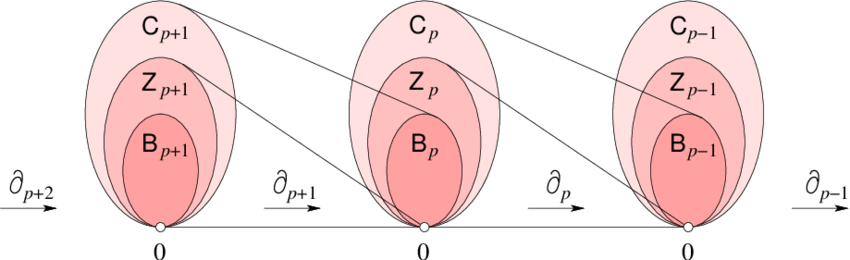
\includegraphics[width=0.8\textwidth]{include/figuras/The-chain-complex-consisting-of-a-linear-sequence-of-chain-cycle-and-boundary-groups.png} 
\caption{Complejo de cadenas representando el grupo de cadenas, el grupo de ciclos y el grupo de bordes. Fuente: \cite{libroEH}}
\label{ref:gruposCadenasOpBorde}
\end{figure}


\subsubsection*{Grupos de homología simplicial}
La idea general de los grupos de homología es poder encontrar los agujeros a partir de los ciclos. Para ello tendremos que ``descartar'' aquellos ciclos que son bordes. Es por esto que cocientaremos el grupo de los ciclos por el grupo de bordes, ya que así todos los bordes serán triviales en homología.

\begin{definition}
Dado un complejo simplicial $K$ se define su \emph{grupo de homología $p$-dimensional} como el cociente
\[
\text{H}_p(K)=\dfrac{\text{Z}_p}{\text{B}_p}
\]
El \emph{número de Betti $p$-dimensional $\beta_p(K)$} como la dimensión de $\text{H}_p(K)$. 
\end{definition}

Luego los elementos $z \in \text{H}_P = \text{H}_p(K)$ son de la forma $z = c + \text{B}_p$ con $c \in \text{Z}_p$, donde $c + \text{B}_p$ es la \emph{clase lateral} de $\text{B}_p$ en $\text{Z}_p$. Dos ciclos $c_1, c_2 \in \text{Z}_p$ representan la misma \emph{clase de homología} $z \in \text{H}_p$ si y sólo si $z= c_1 + \text{B}_p = c_2 + \text{B}_p$; lo que equivale a que $(c_1-c_2) \in \text{B}_p$.

\begin{definition}
Diremos que dos ciclos $c_1, c_2 \in \text{Z}_p$ son \emph{homólogos} si existe $b \in \text{B}_p$ tal que 
\[
c_1 = c_2 + b
\]
\end{definition}

Como $\text{H}_p(K)$ es un grupo finito, por el \emph{teorema de Lagrange} sabemos que el número de clases de homología es
\[
\text{ord } \text{H}_p(K) = \dfrac{\text{ord }  \text{Z}_p}{\text{ord } \text{B}_p}
\]
Además, como $\text{Z}_p$, $\text{B}_p$ y $\text{H}_p$ son espacios vectoriales sobre $\mathbb{Z}_2$ se sigue que 
\[
\beta_p = \text{dim } \text{H}_p = \text{dim } \text{Z}_p - \text{dim } \text{B}_p
\] 

\subsubsection*{Aplicaciones inducidas}
Veremos que una aplicación simplicial entre espacios subyacentes de dos complejos simpliciales lleva ciclos a ciclos y bordes a bordes. Luego, esta aplicación induce una aplicación entre grupos de homología.

Sean $K$ y $L$ complejos simpliciales y $f: K \to L$ una aplicación simplicial. Para cada $p$-símplice $\sigma^p$ se define
\[
f_{\#}(\sigma^p) = 
\begin{cases}
f(\sigma^p)	& \text{ si } \text{dim } f(\sigma^p) = p \\ 
0 			& \text{ en otro caso }
\end{cases}
\]

Puesto que los símplices forman una base de los espacios vectoriales $\text{C}_p(K)$ y $\text{C}_p(L)$, mediante una extensión lineal se obtiene una aplicación lineal $f_{\#}: \text{C}_p(K) \to \text{C}_p(L)$.

\begin{property}
Sean $\partial_K$ y $\partial_L$ los operadores borde de $K$ y $L$ respectivamente. Entonces $f_{\#}\circ \partial_K = \partial_L \circ f_{\#}$ \cite{libroEH}.
\end{property}
La propiedad anterior garantiza que $f_{\#}(\text{Z}_p(K)) \subset \text{Z}_p(L)$ y $f_{\#}(\text{B}_p(K)) \subset \text{B}_p(L)$. Por tanto $f_{\#}$ induce una aplicación lineal $f_{*}: \text{H}_p(K) \to \text{H}_p(L)$, que denominaremos \emph{homomorfismo inducido por $f$}.

Utilizando aproximaciones simpliciales podemos ver que aplicaciones continuas entre poliedros inducen aplicaciones lineales en homología. Para ello definiremos el siguiente operador:

\begin{definition}
\begin{sloppypar}
Sea $K$ un complejo simplicial y consideremos la aplicación ${\lambda: \text{C}_p(K) \to \text{C}_p(\text{Sd}^n\ K)}$ definida sobre los $p$-símplices como
\[
\lambda_p(\sigma^p) = \sum_{\tau^p \in \text{Sd}^n\ \sigma^p} \tau^p
\]
La aplicación $\lambda_p$ se denomina \emph{operador subdivisión}.
\end{sloppypar} 
\end{definition}

\begin{sloppypar}
Sean $K$ y $L$ complejos simpliciales y ${f: \abs{K} \to \abs{L}}$ una aplicación continua y ${g: \text{Sd}^n\ K \to L}$ una aproximación simplicial de $f$. Se define el \emph{homomorfismo inducido} por la aplicación $f$ como la aplicación lineal ${f_{*}: \text{H}_p(K) \to \text{H}_p(L)}$ dada por
\[
f_{*} = g_{*} \circ \lambda_{p*}
\]
Donde $g_{*}$ es el homomorfismo inducido por $g$ y ${\lambda_{p*}: \text{H}_p(K) \to \text{H}_p(\text{Sd}^n\ K)}$ es el isomorfismo inducido por $\lambda_p$.
\end{sloppypar}

\begin{theorem}\label{ref:teoremaHomomorfismoInducido}
Sean $K$ y $L$ dos complejos simpliciales y $f: \abs{K} \to \abs{L}$ un homeomorfismo. Entonces $f_{*}: \text{H}_p(K) \to \text{H}_p(L)$ es un isomorfismo para todo $p$.
\end{theorem}


\subsubsection*{Propiedades topológicas}
En esta sección veremos algunas propiedades topológicas que podemos obtener del estudio de la homología de un complejo simplicial.

\begin{definition}
La característica de Euler de un complejo simplicial $K$ es 
\[
\chi(K) = \sum_{p=0}^{\text{dim } K} (-1)^p s_p
\]
donde $s_p = \text{dim } \text{C}_p(K)$.
\end{definition}
La podremos calcular a partir de los números de Betti:
\begin{theorem}
$\chi(K) = \sum_{p=0}^{\text{dim } K} (-1)^p \beta_p(K)$ \cite{libroEH}.
\end{theorem}

Por el teorema \ref{ref:teoremaHomomorfismoInducido} sabemos que si los espacios subyacentes de dos complejos simpliciales son homeomorfos, entonces sus grupos de homología son isomorfos, y por tanto tendrán la misma dimensión.
\begin{corollary}
\begin{sloppypar}
Sean $K$ y $L$ dos complejos simpliciales tales que $\abs{K} \approx \abs{L}$. Entonces, ${\chi(K)=\chi(L)}$.
\end{sloppypar}
\end{corollary}

Uno de los valores más importantes que obtenemos al calcular los grupos de homología son sus correspondientes números de Betti, ya que estos nos darán mucha información sobre el espacio subyacente. 
\begin{theorem}
Sea $K$ un complejo simplicial. Entonces $\beta_0(K)$ coincide con el número de componentes conexas de $\abs{K}$.
\end{theorem}

\begin{corollary}
$\abs{K}$ es conexo si y sólo si $\beta_0(K)=1$.
\end{corollary}

El \emph{Teorema de dualidad de Alexander} \cite{libroEH} nos permite interpretar los números de Betti de un poliedro contenido en $\mathbb{R}^3$: 
\begin{itemize}
	\item $\beta_0(K)$ nos indica el número de componentes conexas.
	\item $\beta_1(K)$ nos indica el número de túneles.
	\item $\beta_2(K)$ nos indica el número de cavidades.
\end{itemize}

\subsubsection*{Homología singular}
Hay una gran variedad de teorías de homología en topología. La homología que hemos definido es la \emph{homología simplicial}, la cual supone que nuestro espacio ya está expresado como el poliedro subyacente de un complejo simplicial. La \emph{homología singular} generaliza la homología simplicial y permite estudiar otros espacios no triangulables \cite{Crossley_2005}. Este tipo de homología tiene la ventaja que existe para cualquier espacio topológico y que facilita definir conceptos como las aplicaciones inducidas. Sin embargo, los grupos de cadenas singulares tienen dimensión infinita, lo que hace que no sea una buena opción desde el punto de vista computacional. Cabe destacar que, en la mayoría de los casos, sobre todo en dimensiones bajas, la homología singular y simplicial son teorías equivalentes \cite{articuloPersistenciaEH}.

Además, para el \textit{teorema de estabilidad} no nos hará falta hacer uso de la homología singular, ya que se parte de la hipótesis de que el espacio es triangulable.

\subsection{Persistencia}
Introduciremos el concepto de persistencia primero para funciones de una variable. Después veremos en el caso de funciones morse, luego profundizaremos en el caso de los complejos simpliciales y por último para funciones tame. En esta sección seguiré \cite{articuloPersistenciaEH} como referencia.

\subsubsection*{Funciones reales de una variable}
Sea $f: \mathbb{R} \to \mathbb{R}$ una función suave. Recordemos que $x$ es un \emph{punto crítico} y $f(x)$ un \emph{valor crítico de $f$} si $f'(x)=0$. Además, un punto crítico $x$ es \emph{no degenerado} si $f''(x) \neq 0$. Así pues, supongamos que $f$ sólo contiene puntos críticos no degenerados con valores críticos distintos.

Si consideramos el \emph{conjunto de subnivel} $\mathbb{R}_t=f^{-1}(-\infty, t]$ para cada $t \in \mathbb{R}$, entonces veremos que a medida que incrementemos $t$, el número de componentes conexas de $\mathbb{R}_t$ permanecerá constate hasta que pasemos por un $t_0$ valor crítico de $f$. Como podemos ver en la figura \ref{ref:subnivelR}, cuando pasamos por un mínimo local se crea una nueva componente conexa y cuando pasamos por un máximo local se combinan dos componentes conexas en una.

\begin{figure}[!ht]
\centering
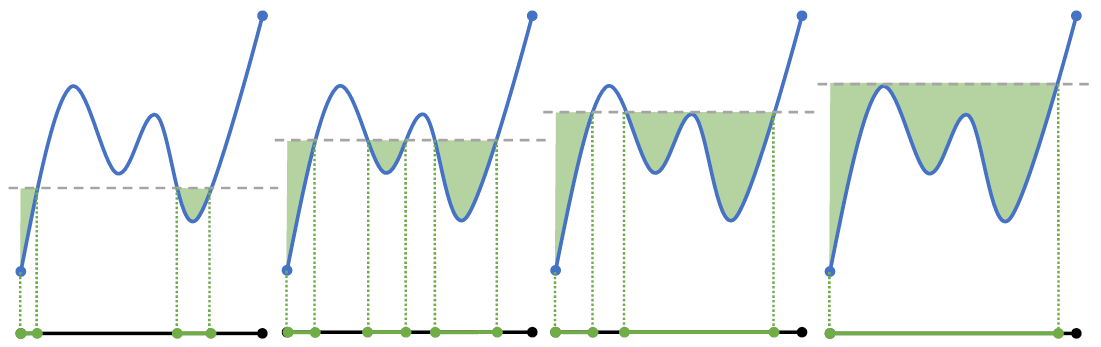
\includegraphics[width=\textwidth]{include/figuras/Sub-level Filtrations.png} 
\caption{Componentes conexas en $\mathbb{R}$ en las diferentes filtraciones. Fuente: \cite{presentacionJustin}}
\label{ref:subnivelR}
\end{figure}

Los puntos críticos de $f$ se emparejan de la siguiente forma: 
\begin{enumerate}
	\item Cuando aparece una nueva componente conexa, diremos que el mínimo local que lo crea \emph{representa} esa componente.  
	\item Cuando pasamos por un máximo local y se juntan dos componentes, emparejamos el máximo con el mayor (el más joven) de los dos mínimos locales que representan dichas componentes. El otro mínimo (el más antiguo) pasa a ser el representante de la nueva componente resultante de juntar las dos anteriores.
\end{enumerate}

Cuando los puntos $x_1$ y $x_2$ se emparejan siguiendo este método, definimos la \emph{persistencia} del par como $f(x_2) - f(x_1)$. Esta persistencia es codificada a través del \emph{diagrama de persistencia}, representando cada par con el punto $(f(x_1),f(x_2))$, como se puede ver en la figura \ref{ref:persistenciaR}. Se puede observar que todos los puntos se encontrarán por encima de la diagonal $y=x$, y que la persistencia es la distancia vertical de un punto a la diagonal. Por razones que explicaremos después se añadirán los puntos de la diagonal al diagrama de persistencia. 

\begin{figure}[!ht]
\centering
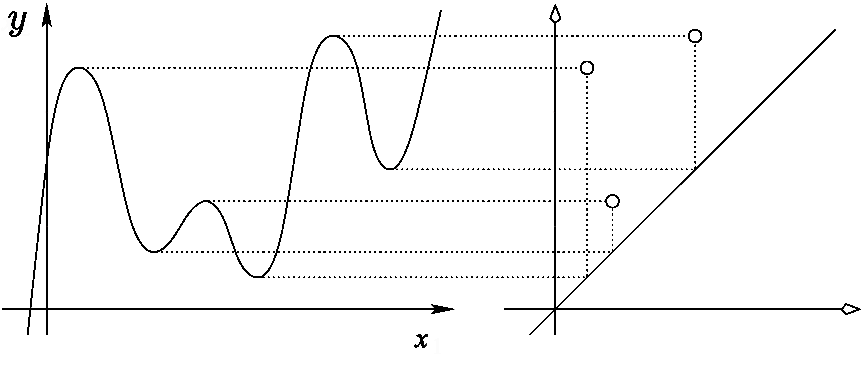
\includegraphics[width=0.8\textwidth]{include/figuras/diagramaR.png} 
\caption{Emparejamiento de los puntos críticos de la función de la función de la izquierda representados como puntos en el diagrama de persistencia de la derecha. Fuente: \cite{articuloPersistenciaEH}}
\label{ref:persistenciaR}
\end{figure}

\subsubsection*{Funciones Morse} 
Vamos a generalizar lo visto con funciones de una variable en $\mathbb{R}$ a funciones suaves sobre \emph{variedades diferenciables} con ciertas propiedades que explicaremos más adelante. Primero recordaremos que son las variedades diferenciables.

\begin{definition}
Una \emph{variedad diferenciable} un espacio topológico $\mathbb{M}$ que satisface:
\begin{enumerate}
	\item $\mathbb{M}$ es Hausdorff ($T_2$).
	\item $\mathbb{M}$ es segundo numerable, es decir, su topología tiene una base numerable.
	\item Todo punto de $\mathbb{M}$ posee un entorno homomorfo a $\mathbb{R}^n$.
	\item Todo punto de $\mathbb{M}$ posee un entorno abierto difeomorfo a $\mathbb{R}^n$.
\end{enumerate}
\end{definition}

Sea $f: \mathbb{M} \to \mathbb{R}$ una aplicación suave. En este caso, un \emph{punto crítico} es un punto $p \in \mathbb{M}$ tal que $\dfrac{\partial f}{\partial x_i}(p)=0$ para $i = 1, ..., n$. Un punto crítico $p$ es \emph{no degenerado} si la matriz Hessiana de las segundas derivadas parciales,
\[
(H_f)_{i,j}=\left(\dfrac{\partial^2 f}{\partial x_i \partial x_j}\right)_{i,j}
\]
es no singular. Si $p$ es un punto crítico no degenerado se define su \emph{índice} como el número de autovalores negativos de la matriz Hessiana en $p$.

\begin{figure}[!ht]
\centering
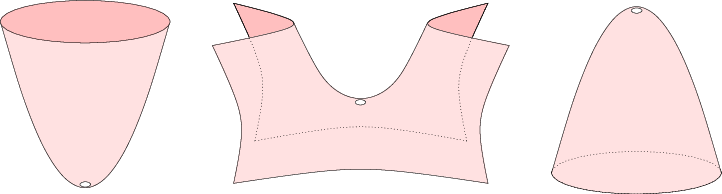
\includegraphics[width=0.7\textwidth]{include/figuras/From-left-to-right-a-minimum-saddle-and-maximum-of-the-vertical-height-function.png} 
\caption{De izquierda a derecha tenemos: un punto crítico no degenerado de índice 0, 1 y 2. Fuente: \cite{articuloPersistenciaEH}}
\label{ref:morseCriticos}
\end{figure}

\begin{definition}
Sea $f: \mathbb{M} \to \mathbb{R}$ una aplicación diferenciable. Diremos que $f$ es una \emph{función Morse} si todos sus puntos críticos son no degenerados y tienen distintos valores críticos.
\end{definition}

\begin{sloppypar}
Se puede demostrar que las funciones Morse poseen un número finito de puntos críticos. Elegimos los valores regulares $t_0 < t_1 < ... < t_m$ tal que existe un único punto crítico ${p_i \in (t_i, t_{i+1})}$ para todo $i = 0, ..., m-1$. Sea $\mathbb{M}_j=f^{-1}(-\infty, t_j]$ el \emph{conjunto de subnivel} que contiene los primeros $j$ puntos críticos.
\end{sloppypar}

Cuando pasamos de $\mathbb{M}_{j-1}$ a $\mathbb{M}_j$ la homología (singular) puede cambiar de dos formas distintas:
\begin{enumerate}[label=\Alph*)]
	\item $\text{H}_p$ incrementa la dimensión en uno, es decir, ${\beta_p(\mathbb{M}_j)} = \beta_p(\mathbb{M}_{j-1}) + 1$.
	\item $\text{H}_{p-1}$ disminuye la dimensión en uno, es decir, ${\beta_{p-1}(\mathbb{M}_j)} = \beta_{p-1}(\mathbb{M}_{j-1}) - 1$.
\end{enumerate}
Donde $p$ es el índice del $j$-ésimo punto crítico. En el primer caso denotaremos a ese punto crítico como \emph{punto crítico positivo} y en el segundo como \emph{punto crítico negativo}.

La persistencia nos dará un emparejamiento de algunos de los puntos críticos positivos de índice $p$ con puntos críticos negativos de índice $p+1$. La idea es determinar el ``momento'' en el que nace una clase de homología y cuando muere, de forma que la persistencia será la diferencia de los tiempos. Para ello haremos uso de funciones entre grupos de homología inducidos por la inclusión de los conjuntos de subnivel $\mathbb{M}_i \subseteq \mathbb{M}_j$ para $i \leq j$. Definiremos de forma más precisa los conceptos de nacimiento y muerte de una clase de homología de la siguiente forma:

\begin{itemize}
	\item Una clase de homología $\alpha$ \emph{nace} en $\mathbb{M}_i$ si no existe en $\mathbb{M}_{i-1}$.
	\item Una clase de homología $\alpha$ nacida en $\mathbb{M}_i$ \emph{morirá al entrar en} $\mathbb{M}_j$ si la imagen de la función inducida por $\mathbb{M}_{i-1} \subseteq \mathbb{M}_{j-1}$ no contiene a la imagen de $\alpha$ pero la imagen de la función inducida por $\mathbb{M}_{i-1} \subseteq \mathbb{M}_j$ si. Siguiendo lo que vimos en funciones de una variable, lo que ocurre es que al entrar en $\mathbb{M}_j$ se junta la clase $\alpha$ con una clase que ya existía en $\mathbb{M}_{i-1}$.
\end{itemize}

Si $\alpha$ nace en $\mathbb{M}_i$ y muere al entrar $\mathbb{M}_j$, entonces emparejaremos sus puntos críticos correspondientes, $x$ e $y$, y diremos que su persistencia es $j-i$ ó $f(y)-f(x)$ según convenga. Esta persistencia es codificada a través de los \emph{diagramas de persistencia}, $\text{Dgm}_p(f)$, representando cada emparejamiento de un punto crítico positivo de índice $p$ con un punto crítico negativo de índice $p+1$ añadiendo el punto $(f(x),f(y))$ al diagrama. Al igual que hicimos en el caso de funciones reales de una variable, añadiremos los puntos de la diagonal en el diagrama de persistencia.

\subsubsection*{Funciones tame}
Se puede comprobar que las funciones Morse sobre variedades diferenciables limitarán demasiado para algunas aplicaciones. Es por ello que consideraremos un tipo de función $f: \mathbb{X} \to \mathbb{R}$, donde $f$ y $\mathbb{X}$ cumplen una serie de propiedades menos restrictivas. Empezaremos extendiendo la noción de punto crítico de la siguiente forma:

\begin{definition}
\begin{sloppypar}
Sea $\mathbb{X}$ un espacio topológico, $f$ una función real en $\mathbb{X}$ y ${\mathbb{X}_t=f^{-1}(-\infty, t]}$ el conjunto de subnivel definido para el valor $t$. Un \emph{valor crítico de homología} de $f$ es un número real $a$ para el cual existe un entero $k$ tal que para todo $\epsilon > 0$ lo suficientemente pequeño, la función $\text{H}_k(\mathbb{X}_{a-\epsilon}) \to \text{H}_k(\mathbb{X}_{a+\epsilon})$ inducida por la inclusión, $\mathbb{X}_{a-\epsilon} \subseteq \mathbb{X}_{a+\epsilon}$, no es un isomorfismo.
\end{sloppypar}
\end{definition}

En otras palabras, los valores críticos de homología son los niveles en los cuales cambia la homología de los conjuntos de subnivel. Como ya hemos visto, en el caso de las funciones Morse, estos puntos críticos de homología coinciden con los valores críticos de la función.


\begin{definition}
Una función $f: \mathbb{X} \to \mathbb{R}$ es \emph{tame} si los grupos de homología de cada subnivel son finito-dimensionales y tienen un número finito de valores críticos de homología.
\end{definition}

\begin{sloppypar}
En particular, las funciones morse sobre variedades compactas son funciones tame, porque poseen un número finito de puntos críticos. Para poder simplificar la notación, para cada entero $k$ fijo, escribimos ${F_x = \text{H}_k(f^{-1}(-\infty, x])}$, y para $x < y$, denotamos como ${\tensor*{f}{*^{y}_{x}}: F_x \to F_y}$ la aplicación lineal inducida por la inclusión $\mathbb{X}_{x} \subseteq \mathbb{X}_{y}$. Una vez definida la notación, observaremos el lema \ref{ref:lemaValCritico}, el cual nos será de gran ayuda para la demostración del \emph{teorema de estabilidad}.
\end{sloppypar}

\begin{property}
La familia de aplicaciones $(F_{x}^{y})_{x \leq y}$ satisface las siguientes propiedades:
\begin{itemize}
	\item $f_{x}^{x}= \text{id}_{F_x}$.
	\item $f_{m}^{y} \circ f_{x}^{m} = f_{x}^{y}$, con $x \leq m \leq y$.
\end{itemize}
\end{property}


\begin{lemma}[Lema del valor crítico]
\label{ref:lemaValCritico}
Si un intervalo cerrado $[x, y]$ no contiene ningún valor crítico de homología de $f$, entonces $f_{x}^{y}$ es un isomorfismo para todo entero $k$.
\end{lemma}

\begin{proof}
Sea $m = \dfrac{x+y}{2}$, tenemos que $f_{x}^{y}=f_{m}^{y} \circ f_{x}^{m}$. Supongamos que $f_{x}^{y}$ no es un isomorfismo; por lo tanto, al menos una de las funciones $f_{m}^{y}$ y $f_{x}^{m}$ no es un isomorfismo.\\
Por inducción sobre las funciones no isomorfas de la composición, obtenemos una sucesión de intervalos encajados cerrados y acotados, $I_n=[x_n,y_n]$, tal que
\[
\lim_{x\to\infty} \abs{y_n - x_n} = 0 \text{ y } f_{x_n}^{y_n} \text{ no es un isomorfismo para todo  } n \in \mathbb{N}
\]
por lo que, aplicando el principio de intervalos encajados en $\mathbb{R}$, sabemos que su intersección es un punto $a \in \mathbb{R}$, que verifica que $f_{a-\epsilon}^{a+\epsilon}$ no es un isomorfismo para todo $\epsilon > 0$. Luego, el punto $a$ es un valor crítico de homología en $[x, y]$, contradiciendo nuestra hipótesis inicial.
\end{proof}

\begin{definition}
Sea ${f_{x}^{y}: F_x \to F_y}$ la aplicación lineal inducida por la inclusión $\mathbb{X}_{x} \subseteq \mathbb{X}_{y}$. Se define los \emph{grupos de homología persistente} como la imagen de $F_x$ en $F_y$ de la aplicación $f_{x}^{y}$, es decir,
\[
F_{x}^{y} = \text{im } f_{x}^{y}
\]
Los correspondientes \emph{números de Betti persistentes} se definen como los rangos de estos grupos, es decir, $\beta_{x}^{y} = \text{dim } F_{x}^{y}$, para todo $-\infty \leq x \leq y \leq + \infty$. 
\end{definition}
Por convención, se establece que $F_{x}^{y}= \{0\}$ cuando $x$ ó $y$ son infinito. El grupo de homología persistente consiste de las clases que han nacido antes de $x$ y siguen vivas en $y$.


\begin{remark}
Si analizamos las aplicaciones $f_{x}^{y}$, observamos que el $\text{ker } f_{x}^{y}$ son aquellos elementos $\gamma \in F_x$ tales que $f_{x}^{y}(\gamma)=0$. Esto significa que si $c$ es un ciclo representando a $\gamma$, $c \in \text{B}_k(\mathbb{X}_y)$. Como consecuencia
\[
\text{ker } f_{x}^{y} = \dfrac{\text{Z}_k(\mathbb{X}_x) \cap \text{B}_k(\mathbb{X}_y)}{\text{B}_k(\mathbb{X}_x)}
\]
para cada dimensión $k$ fija. 
\end{remark}

Sea $f: \mathbb{X} \to \mathbb{R}$ una función tame, $(a_i)_{i=1..n}$ sus valores críticos homológicos y se considera la secuencia entrelazada $(b_i)_{i=0..n}$, tal que $b_{i-1} < a_{i} < b_{i}$ para $1 \leq i \leq n$. Para capturar la homología que existe en el principio y el final establecemos $b_{-1} = a_0 = -\infty$ y $b_{n+1} = a_{n+1} = +\infty$. Entonces,
\begin{definition}
Se define la multiplicidad del par $(a_i, a_j)$ como
\[
\mu_{i}^{j} = \beta_{b_{i-1}}^{b_j} - \beta_{b_i}^{b_j} +  \beta_{b_i}^{b_{j-1}} - \beta_{b_{i-1}}^{b_{j-1}} \text{, para todo } i, j \in \mathbb{Z} \text{ tal que } 0 \leq i < j \leq n+1
\]
\end{definition}

Podemos visualizar la multiplicidad, $\mu_{i}^{j}$, como se muestra en la figura \ref{ref:multiplicidadDiagrama}. Donde, considerando $\beta_{x}^{y}$ como una función sobre el plano real extendido $\overline{\mathbb{R}}^2$, donde $\overline{\mathbb{R}} = \mathbb{R} \cup \{-\infty, +\infty\}$; entonces, $\mu_{i}^{j}$ es la suma alternada de los número de Betti persistentes en las esquinas del cuadrado $[b_{i-1}, b_i]\times[b_{j-1}, b_j]$.

\begin{figure}[!ht]
\centering
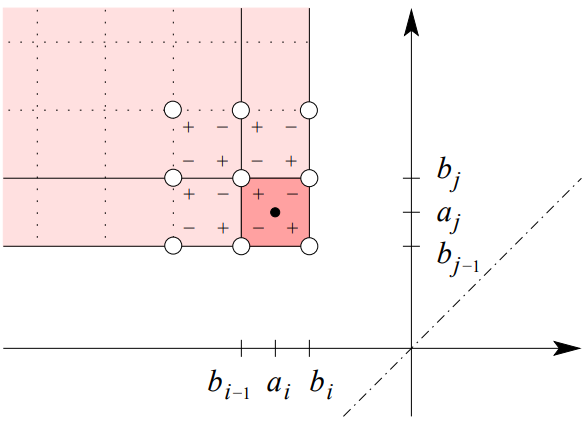
\includegraphics[width=0.5\textwidth]{include/figuras/multiplicidadEsquinas.png} 
\caption{La multiplicidad del punto $(a_i, a_j)$ es la suma alternada de los número de Betti persistentes en las esquinas del cuadrado $[b_{i-1}, b_i]\times[b_{j-1}, b_j]$. Fuente: \cite{Cohen-Steiner2007}}
\label{ref:multiplicidadDiagrama}
\end{figure}

\begin{remark}
Si $x$ y $x'$ se encuentran dentro del intervalo $(a_i, a_{i+1})$, y $y$ e $y'$ en el intervalo $(a_{j-1}, a_j)$, entonces $\beta_{x}^{y} = \beta_{x'}^{y}$. Este resultado se sigue de que, debido al \emph{Lema del valor crítico}, $F_{x}^{y}$ y $F_{x'}^{y'}$ son isomorfos.
\end{remark}

\begin{definition}
El \emph{diagrama de persistencia} $\text{Dgm}(f) \subset \overline{\mathbb{R}}^2$ de $f$ es el multiconjunto de puntos $(a_i, a_j)$ con multiplicidad $\mu_{i}^{j}$ para todo $0 \leq i < j \leq n+1$, unión los puntos de la diagonal, $\Delta=\{(x, y) \in \overline{\mathbb{R}}^2 \mid y = x\}$, con multiplicidad infinito.
\end{definition}

Denotaremos por $\#(A)$ la \emph{multiplicidad total} de un multiconjunto $A$, el cual, por definición es la suma de las multiplicidades de los elementos de $A$. Por lo tanto, la multiplicidad total del diagrama de persistencia menos la diagonal es
\[
\#(\text{Dgm}(f) \setminus \Delta) = \sum_{i < j} \mu_{i}^{j}
\]
la cual es llamada \emph{tamaño} del diagrama de persistencia.

Denotaremos el cuadrante superior izquierda cerrado con vértice en el punto $(x, y)$ como $Q_{x}^{y} = [-\infty, x] \times [y, \infty]$.

\begin{lemma}[Lema del $k$-Triángulo]
Sea $f$ una función tame y suponemos que $x < y$ son diferentes de los valores críticos homológicos de $f$. Entonces la multiplicidad total del diagrama de persistencia en en cuadrante superior izquierda con vértice $(x, y)$ es
\[
\#(Dgm(f) \cap Q_{x}^{y})= \beta_{x}^{y}
\]
\end{lemma}

\begin{proof}
Podemos asumir sin perder generalidad, que $x = b_i$ y $y = b_{j-1}$. Por definición, la multiplicidad total en el cuadrante superior izquierda es igual a la suma de las multiplicidades de los puntos contenidos en dicho cuadrante, luego
\[
\#(Dgm(f) \cap Q_{x}^{y}) = \sum_{k \leq i} \sum_{l > j}  \mu_{k}^{l} =
\sum_{k \leq i} \sum_{l > j} (\beta_{b_{k-1}}^{b_l} - \beta_{b_k}^{b_l} + \beta_{b_k}^{b_{l-1}} - \beta_{b_{k-1}}^{b_{l-1}})
\]
Como se muestra en la figura \ref{ref:multiplicidadDiagrama}, cuando se suman las multiplicidades, ocurre la cancelación entre signos positivos y negativos de las esquinas de los cuadrados. Entonces:
\begin{gather*}
\#(Dgm(f) \cap Q_{x}^{y}) = \beta_{b_{-1}}^{b_{n+1}} - \beta_{b_{i}}^{b_{n+1}} + \beta_{b_i}^{b_{j-1}} - \beta_{b_{-1}}^{b_{j-1}} =\\
= \beta_{-\infty}^{+\infty} - \beta_{b_{i}}^{+\infty} + \beta_{b_i}^{b_{j-1}} - \beta_{-\infty}^{b_{j-1}} = \beta_{b_i}^{b^{j-1}} = \beta_{x}^{y}
\end{gather*}
ya que $F_{x}^{y}= \{0\}$ cuando $x$ ó $y$ son infinito, y por lo tanto su dimensión, es decir, su número de Betti persistente, es cero.
\end{proof}

Este lema nos garantiza que el diagrama de persistencia codifica toda la información sobre los grupos de homología persistente \cite{libroEH}.

\subsubsection*{Persistencia en complejos simpliciales}
Veremos que podemos particularizar la persistencia vista para funciones tame a complejos simpliciales. Para ello utilizaremos las \emph{filtraciones} de un complejo simplicial como conjuntos de subnivel.

\begin{definition}
Sea un complejo simplicial $K$ y $f: K \to \mathbb{R}$ una función. Entonces, $f$ será \emph{monótona} si $f(\sigma) \leq f(\tau)$ si $\sigma$ es una cara de $\tau$.
\end{definition}
\begin{sloppypar}
La monotonía de $f$ garantiza que para cada $a \in \mathbb{R}$, el conjunto de subnivel ${K(a) = f^{-1}(-\infty,a]}$ es un subcomplejo de $K$.
\end{sloppypar}


\begin{definition}
Sean $a_1 < a_2 < ... < a_n$ los valores que toma la función en los símplices y sea $a_0 = -\infty$. Entonces $f$ induce una \emph{filtración}
\[
\emptyset = K_0 \subset K_1 \subset ... \subset K_n = K, \text{ con } K_i=K(a_i)
\]
\end{definition}
Estas filtraciones pueden ser obtenidas de diversas formas. Por un lado, podremos obtener filtraciones variando el radio de los complejos de \v{C}ech, Vietoris-Rips y alfa complejos; y más adelante veremos como obtener filtraciones de complejos simpliciales más generales a partir de la filtración de las estrellas inferiores de una función PL.

De esta forma, al igual que vimos en las funciones Morse, una clase de homología $\alpha$ nace en $K_i$ si no está en la imagen de la función inducida por la inclusión $K_{i-1} \subset K_i$. Además, una clase $\alpha$ que nace en $K_i$ muere al entrar en $K_j$ si la imagen de la función inducida por $K_{i-1} \subset K_{j-1}$ no contiene la imagen de $\alpha$, pero la imagen de la función inducida por $K_{i-1} \subset K_j$ sí.

Introduciremos los grupos de homología persistente, reduciendo la notación de la siguiente forma: $F_i = F_{b_i}$, $F_{i}^{j}=F_{b_i}^{b_j}$ y $\beta_{i}^{j}=\beta_{b_i}^{b_j}$. Así podemos redefinir la noción de nacimiento y muerte de una clase de homología como sigue
\begin{itemize}
	\item Una clase $\gamma \in F_i$ \emph{nace} en $K_i$ si $\gamma \notin F_{i-1}^{i}$.
	\item Una clase $\gamma \in F_i$ nacida en $K_i$ \emph{muere} al entrar en $K_j$ si $f_{i}^{j-1}(\gamma)\notin F_{i-1}^{j-1}$, pero $f_{i}^{j}(\gamma)\notin F_{i-1}^{j}$. 
\end{itemize} 

\begin{definition}
Sea $\gamma$ una clase de homología que nace en $K_i$ y muere al entrar en $K_j$. Se define la \emph{persistencia} de $\gamma$ como $\text{pers}(\gamma)= a_j - a_i$. Asimismo, la diferencia $j-i$ se denomina \emph{índice de persistencia} de la clase $\gamma$. Si una clase $\gamma$ nace en $K_i$ pero nunca muere, entonces diremos que su persistencia, al igual que su índice, es infinito.
\end{definition}

Siguiendo esta notación, se define la multiplicidad como
\[
\mu_{i}^{j} = (\beta_{i}^{j-1}-\beta_{i}^{j})-(\beta_{i-1}-\beta_{i-1}^{i})
\]
Donde a $\beta_{i}^{j-1}$ se puede interpretar como el número de clases de homología que están vivas en $K_i$ y siguen vivas en $K_{j-1}$. Por lo tanto, la primera diferencia de la igualdad se interpreta como el número de clases independientes que están vivas en $K_i$ y mueren en $K_j$; mientras que la segunda diferencia son el número de clases independientes que nacen antes de $K_i$ y mueren en $K_j$. En conclusión, la multiplicidad, $\mu_{i}^{j}$, se interpreta como el número de clases de homología que nacen en $K_i$ y mueren en $K_j$.

\begin{figure}[!ht]
\centering
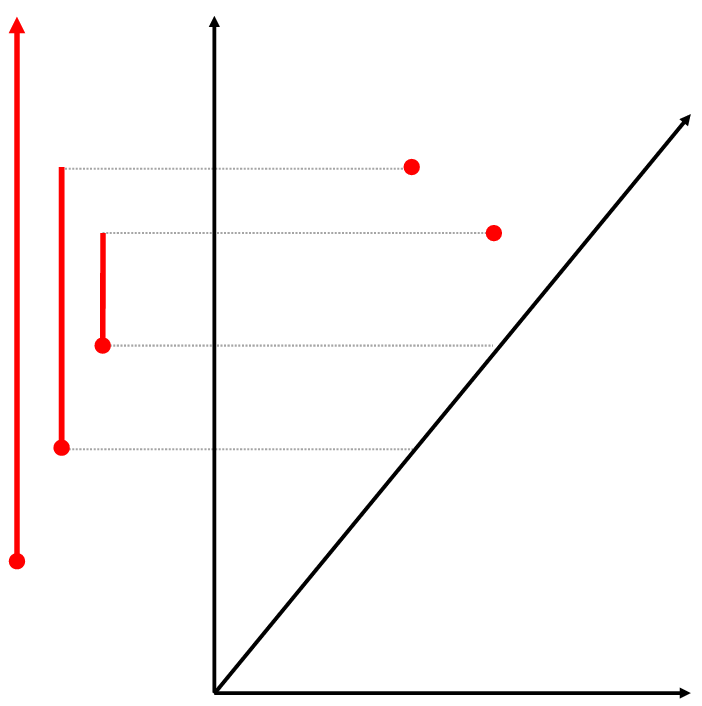
\includegraphics[width=0.35\textwidth]{include/figuras/The-Persistence-Diagram-Associated-to-a-Barcode.png} 
\caption{Código de barras asociado a un diagrama de persistencia. Fuente: \cite{articuloJustin}}
\label{ref:codigoBarras}
\end{figure}

Cada punto $(a_i, a_j)$ representa $\mu_{i}^{j}$ clases de homología independientes cuya persistencia coincide con la distancia del punto $(a_i, a_j)$ a su proyección vertical sobre la diagonal $\Delta$. Por razones técnicas, los puntos de la diagonal se añaden al diagrama de persistencia con multiplicidad infinito.

Adicionalmente de los diagramas de persistencia, podemos codificar la información sobre la homología persistente a través de los denominados \emph{códigos de barras}. Estas representaciones se pueden obtener a partir del diagrama de persistencia dibujando por cada punto $(a_i, a_j)$ con $a_i < a_j$ de dicho diagrama $\mu_{i}^{j}$ intervalos semiabiertos $[a_i, a_j)$, como se muestra en la figura \ref{ref:codigoBarras}.

\subsubsection*{Funciones PL}
Un caso especial de las funciones tame son las \emph{funciones lineales a trozos} (en inglés: \emph{piecewise linear function}) la cuales asocian el espacio subyacente de un complejo simplicial a valores reales.

\begin{definition}
Sea $K$ un complejo simplicial con valores reales asignados en todos sus vértices. Se define la función lineal a trozos $f: \abs{K} \to \mathbb{R}$ como la extensión linear de los valores de los vértices sobre los símplices, es decir,
\[
f(x)=\sum_{i} b_i(x)f(u_i)
\]
donde $u_i$ son los vértices de $K$ y $b_i(x)$ son las coordenadas baricéntricas de $x$.
\end{definition}
Por simplicidad se asume que $f\vert_{\text{Vert }K}$ es inyectiva. Reindexando los vértices de forma que $f(u_i) < f(u_2) < ... < f(u_n)$, definimos $K_i$ como el subcomplejo  definifo por los primero $i$ vértices.

\begin{definition}
La \emph{estrella inferior} es el subconjunto de símplices para los cuales $u_i$ es el vértice de mayor valor de $f$:
\[
\text{St}\_u_i = \{\sigma \in \text{St }u_i \mid x \in \sigma \Rightarrow f(x) \leq f(u_i)\}
\] 
\end{definition}

Como ocurría con la estrella, la estrella inferior generalmente no es un subcomplejo. Añadiendo las caras restantes al conjunto, obtenemos la \emph{estrella inferior cerrada}, la cual es un subcomplejo de $K$. Debido a la asunción de la inyectividad de la restricción de $f$ a sus vértices, cada símplice tiene un único vértice con valor máximo, y por tanto pertenece a una única estrella inferior. Luego, $K_i$ es la unión de las primeras $i$ estrellas inferiores; obteniendo la siguiente filtración de $K$:

\begin{definition}
Sea $K$ un complejo simplicial con valores reales asignados en todos sus vértices y $f$ una función PL sobre $K$. Entonces definimos la \emph{filtración de las estrellas inferiores de $f$} como la cadena de complejos $\emptyset = K_0 \subseteq K_1 \subseteq ... \subseteq K_n = K$, donde $K_i=K_{i-1} \cup \text{St}\_u_i$. 
\end{definition}

Esta filtración cumple las siguientes propiedades:
\begin{property}
$K_i$ tiene el mismo tipo de homotopía que el subnivel $\abs{K}_t=f^{-1}(-\infty, t]$, para todo $f(u_i) \leq t < f(u_{i+1})$ \cite{libroEH}.
\end{property}

\begin{property}
\begin{sloppypar}
La la variación de la homología en los conjuntos de subnivel ${\abs{K}_t=f^{-1}(-\infty, t]}$ es la misma que la homología de la filtración de las estrellas inferiores de $f$.
\end{sloppypar}
\end{property}

\begin{property}
Sea $\mathbb{X}$ un espacio topológico triangulable. Entonces podemos aproximar toda función tame en $\mathbb{X}$ a partir de una función PL en su triangulación \cite{articuloPersistenciaEH}.
\end{property}




